\documentclass[a4paper,11pt]{report}

% We need more TeX registers
\usepackage{etex}
\usepackage[utf8]{inputenc}

\usepackage[a4paper, asymmetric, right=2.5cm, left=3.0cm, top=2.5cm, bottom=2.0cm]{geometry}

\usepackage[german, english]{babel}
\usepackage[left]{eurosym}
\usepackage{tabularx}
\newcolumntype{v}[1]{%
  >{\raggedright\hspace{Opt}}p{#1}%
}
\usepackage{slashbox}

\usepackage{tikz}
\usetikzlibrary{arrows}
\usetikzlibrary{shapes}
\usetikzlibrary{plotmarks}
\usetikzlibrary{decorations}
\usetikzlibrary{backgrounds,positioning}
\usepackage{amsmath}
\usepackage{amsfonts}
\usepackage{amssymb}
\usepackage{makeidx}
%\usepackage{multind}
\usepackage{tocbibind}
\usepackage{nicefrac}
\usepackage{thumbpdf}


\usepackage[draft=false, plainpages=false,
						colorlinks=true, linkcolor=blue, citecolor=blue, urlcolor=red,
						bookmarks, bookmarksopen, bookmarksopenlevel=1, bookmarksnumbered=true,breaklinks=true,
						pdftitle={The GrGen User Manual},
						pdfauthor={Jakob Blomer, Rubino Geiss, Edgar Jakumeit},
						pdfkeywords={
						graph, graph transformation, graph rewriting, tool, spo, manual, grgen, graph rewrite generator,
						University of Karlsruhe, IPD Goos},
						pdfpagelabels
						]{hyperref}

\usepackage[all]{xy}
\usepackage{xcolor}
\definecolor{light}{gray}{0.8}
\definecolor{tuerkis}{cmyk}{0.5,0.15,0,0.3}
\usepackage{picins} %wrapfig and floatflt suck deeply
\usepackage{graphicx}
\usepackage{calc}
\usepackage{xspace}

%\usepackage{listings}
%\lstset{language=C, numbers=left, numberstyle=\tiny, stepnumber=5}

\providecommand{\O}[1]{\ensuremath{\mathcal{O}\left( #1 \right)}}

\providecommand{\N}{\ensuremath{\mathbb{N}}}
\providecommand{\Z}{\ensuremath{\mathbb{Z}}}
\renewcommand{\P}{\ensuremath{\mathbb{P}}}
\providecommand{\F}{\ensuremath{\mathbb{F}}}
\providecommand{\Q}{\ensuremath{\mathbb{Q}}}
\providecommand{\R}{\ensuremath{\mathbb{R}}}
\providecommand{\C}{\ensuremath{\mathbb{C}}}

\providecommand{\abs}[1]{\left\lvert #1 \right\rvert}
\providecommand{\norm}[1]{\left\lVert #1 \right\rVert}
\providecommand{\floor}[1]{\left\lfloor #1 \right\rfloor}
\providecommand{\svert}{\; \vert \;}

\DeclareMathOperator{\Abb}{Abb}   % Abbildungsmenge
\DeclareMathOperator{\Sym}{Sym}   % Bijektionenmenge
\DeclareMathOperator{\Hom}{Hom}   % Homomorphismenmenge
\DeclareMathOperator{\End}{End}   % Endomorphismenmenge
\DeclareMathOperator{\Aut}{Aut}   % Automorphismenmenge
\DeclareMathOperator{\deF}{def}
\DeclareMathOperator{\ran}{ran}
\DeclareMathOperator{\lhs}{lhs}
\DeclareMathOperator{\rhs}{rhs}

\providecommand{\id}{\ensuremath{\textsf{id}}}  % identische Abbildung
\DeclareMathOperator{\Kern}{Kern}     % Kern
\DeclareMathOperator{\Bild}{Bild}     % Bild

\providecommand{\Bin}[2]{\ensuremath{\operatorname{Bin} \left( #1 , #2 \right)}}
\providecommand{\Hyp}[2]{\ensuremath{\operatorname{Hyp} \left( #1 , #2 \right)}}

\providecommand{\PeroW}[2]{\ensuremath{\text{Per}^{#1}_{#2}\text{(oW)}}}
\providecommand{\PermW}[2]{\ensuremath{\text{Per}^{#1}_{#2}\text{(mW)}}}
\providecommand{\KomoW}[2]{\ensuremath{\text{Kom}^{#1}_{#2}\text{(oW)}}}
\providecommand{\KommW}[2]{\ensuremath{\text{Kom}^{#1}_{#2}\text{(mW)}}}

\makeatletter
\def\Relbar{\mathrel{\smash=}}
\def\Leftarrowfill@{\arrowfill@\Leftarrow\Relbar\Relbar}
\def\Rightarrowfill@{\arrowfill@\Relbar\Relbar\Rightarrow}
\newcommand{\xRightarrow}[2][]{\ext@arrow 0359\Rightarrowfill@{#1}{#2}}
\newcommand{\xLeftarrow}[2][]{\ext@arrow 3095\Leftarrowfill@{#1}{#2}}
\makeatother

\usepackage{rail}
\railalias{lbrace}{\{}
\railalias{rbrace}{\}}
\railalias{underscore}{\_}
\railalias{dollar}{\$}
\railalias{percent}{\%}
%\railalias{ampersand}{<>}
\railalias{backslash}{\char"5C}
\railalias{tilde}{$\sim$}
\railalias{titilde}{$\sim\sim$}
\railalias{ampersand}{\&}
\railalias{doubleampersand}{\&\&}
\railalias{etc}{$\cdots$}
\railalias{xorhat}{$\wedge$}
\railalias{railat}{@}

\railalias{analyzegraph}{analyze\_graph}
\railalias{gensearchplan}{gen\_searchplan}
\railalias{setmaxmatches}{set\_max\_matches}
\railalias{dumpsourcecode}{dump\_sourcecode}

\railterm{lbrace,rbrace,dollar,percent,ampersand,backslash,underscore,tilde,ampersand,analyzegraph,gensearchplan,setmaxmatches,dumpsourcecode,doubleampersand,xorhat}

\usepackage[final]{listings}

\usepackage{soul}
\usepackage{titlesec}
\usepackage{titletoc}
\usepackage{fancyhdr}
\usepackage{subfig}

\usepackage{examplep}

% sectionreformatting
% tableofcontents level == 3 (subsubsection)
\setcounter{tocdepth}{3}
\setcounter{secnumdepth}{3}

% Headings
\pagestyle{myheadings}

\renewcommand{\chaptermark}[1]{\markboth{\it #1}{}}
\renewcommand{\sectionmark}[1]{\markright{\thesection \; \it #1}}
\lhead[\fancyplain{}{\thepage}]%
      {\fancyplain{}{\rightmark}}
\rhead[\fancyplain{}{\leftmark}]%
  {\fancyplain{}{\thepage}}
\renewcommand{\headrulewidth}{0pt}

\capsdef{////}{\upshape}{0.125em}{0.4583em}{0.5833em}
\newcommand{\versal}[1]{\MakeUppercase{\caps{#1}}}

% Other desccription labels, not that ugly bold font
% And put the description on a line of its own
\renewcommand\descriptionlabel[1]{%
  \hspace\labelsep {% local changes only
    \advance\linewidth\leftmargin
    \advance\linewidth-\labelsep
    \makebox[\linewidth][l]{\it #1}}}

% Other TOC headings for chapters \contentslabel{2.3em}}
%\titlecontents{chapter}[0em]{\sf\vspace*{2ex}}{Kapitel
%          \thecontentslabel{} --- }
%          {}{\hfill\contentspage\vspace*{1ex}}

\titlecontents{part}[0em]{\sf\large\vspace*{2ex}}{\contentslabel{2.3em}}
              {}{\hfill\contentspage\vspace*{1ex}}

\titlecontents{chapter}[0em]{\sf\vspace*{2ex}}{\contentslabel{2.3em}}
              {}{\hfill\contentspage\vspace*{1ex}}

%\titlecontents{chapter}[1.5em]{\sf}{2.3em}{1pc}{}{}{}
\dottedcontents{section}[3.8em]{}{2.3em}{1pc}

% Other formatting of chapter and section headings
\newcommand*\chaptitle[1]{\Large\filleft\versal{#1}}


\titleformat{\part}[block]
    {\LARGE\sf}
  {\versal{TEIL}\hspace*{2ex}\thepart}
  {4ex}{\Huge\newline\newline\centering}
\titleformat{\chapter}[display]
  {\large\sf}
  {\filright\versal{\chaptertitlename}\hspace*{2ex}\thechapter}
  {4ex}{\chaptitle}
\titleformat{\section}
  {\large\sf}{\thesection}
  {1em}{}
\titleformat{\subsection}
  {\sf}{\thesubsection}
  {1em}{}
\titleformat{\subsubsection}
  {\sf}{\thesubsubsection}
  {1em}{}
\titleformat{\paragraph}
  {\sf}{\theparagraph}{0em}{}
\titlespacing*{\paragraph}{0cm}{2.75ex plus 1ex minus .2ex}{.5em}

\makeatletter
\renewcommand*{\tableofcontents}{%
  \begingroup
    \@restonecolfalse
    \expandafter\chapter\expandafter*\expandafter{\contentsname}%
    \@mkboth{\contentsname}{\contentsname}%
    \@starttoc{toc}%
  \endgroup
} \makeatother



\selectlanguage{english}
\lstdefinelanguage{grgenmodel}
  {morekeywords={model, class, edge, node, connect, extends},
   sensitive=true,
   morecomment=[l]{\#},
  }
\lstdefinelanguage{grgenactions}
  {morekeywords={actions, using, rule, pattern, replace, negative},
   sensitive=true,
   morecomment=[l]{\#},
  }
\lstdefinelanguage{grshell}
  {morekeywords={},
   sensitive=true,
   morecomment=[l]{\#},
  }
\lstset{numbers=left, numberstyle=\tiny, stepnumber=1, firstnumber=auto, frame=single}
\providecommand{\GrG}{{\scshape GrGen}}
\newcommand{\lined}{\hfill \hrule\hfill\vspace{1mm} \\}

\title{\GrG\ User Manual \\ Graph Rewrite System}
\author{Jakob Blomer \\ \\ Institut für Programmstrukturen und Datenorganisation\\
Fakultät für Informatik\\
Universität Karlsruhe (TH)}

\begin{document}

\maketitle

\tableofcontents

\chapter{System Overview}

\GrG\ is a generative programming system for graph rewriting. \GrG\ is mainly designed for \emph{typed graphs}.  That means, graphs are not only nodes and edges, but labeled (\emph{attributed typed}) directed multigraphs. The type system is specified as class hierarchy, like a classes in object oriented languages. Type systems for specific sets of graphs can be specified by user supplied graph meta models. Such a graph model describes a set of well-formed graphs, i.e.\ allowed node and edge types, their attributes and specific connection assertions. We'll build a graph model for a turing machine in section \ref{anexample}.

How does graph rewriting work? \GrG\ implements an SPO-based approach. Given a host graph $H$, each \emph{rewriting rule} $p: L \longrightarrow R$ consists of a pattern $L$ and a transformation specification $R$ in form of a adopted pattern graph. The process of rewriting searches a match $H_L \unlhd H$ (i.e.\ a graph homomorphism from $L$ to a subgraph of $H$) and rewrites $H_L$ to $R$. Nodes or edges added to $R$ (in compare to $L$) will be added $H_L$ and nodes or edges deleted in $R$ will be deleted in $H_L$. The homomorphism may not be unique.

We'll have a look at a small example. First we use a special case to construct our host graph: an empty pattern does always produce exactly one match (independently of the host graph). So starting with an empty host graph $H$ we construct an apple using
\[ p:  \begin{array}[c]{c} 
\includegraphics[width=3cm]{fig/empty} \end{array} \begin{array}[c]{c} \longrightarrow \end{array} \begin{array}[c]{c} 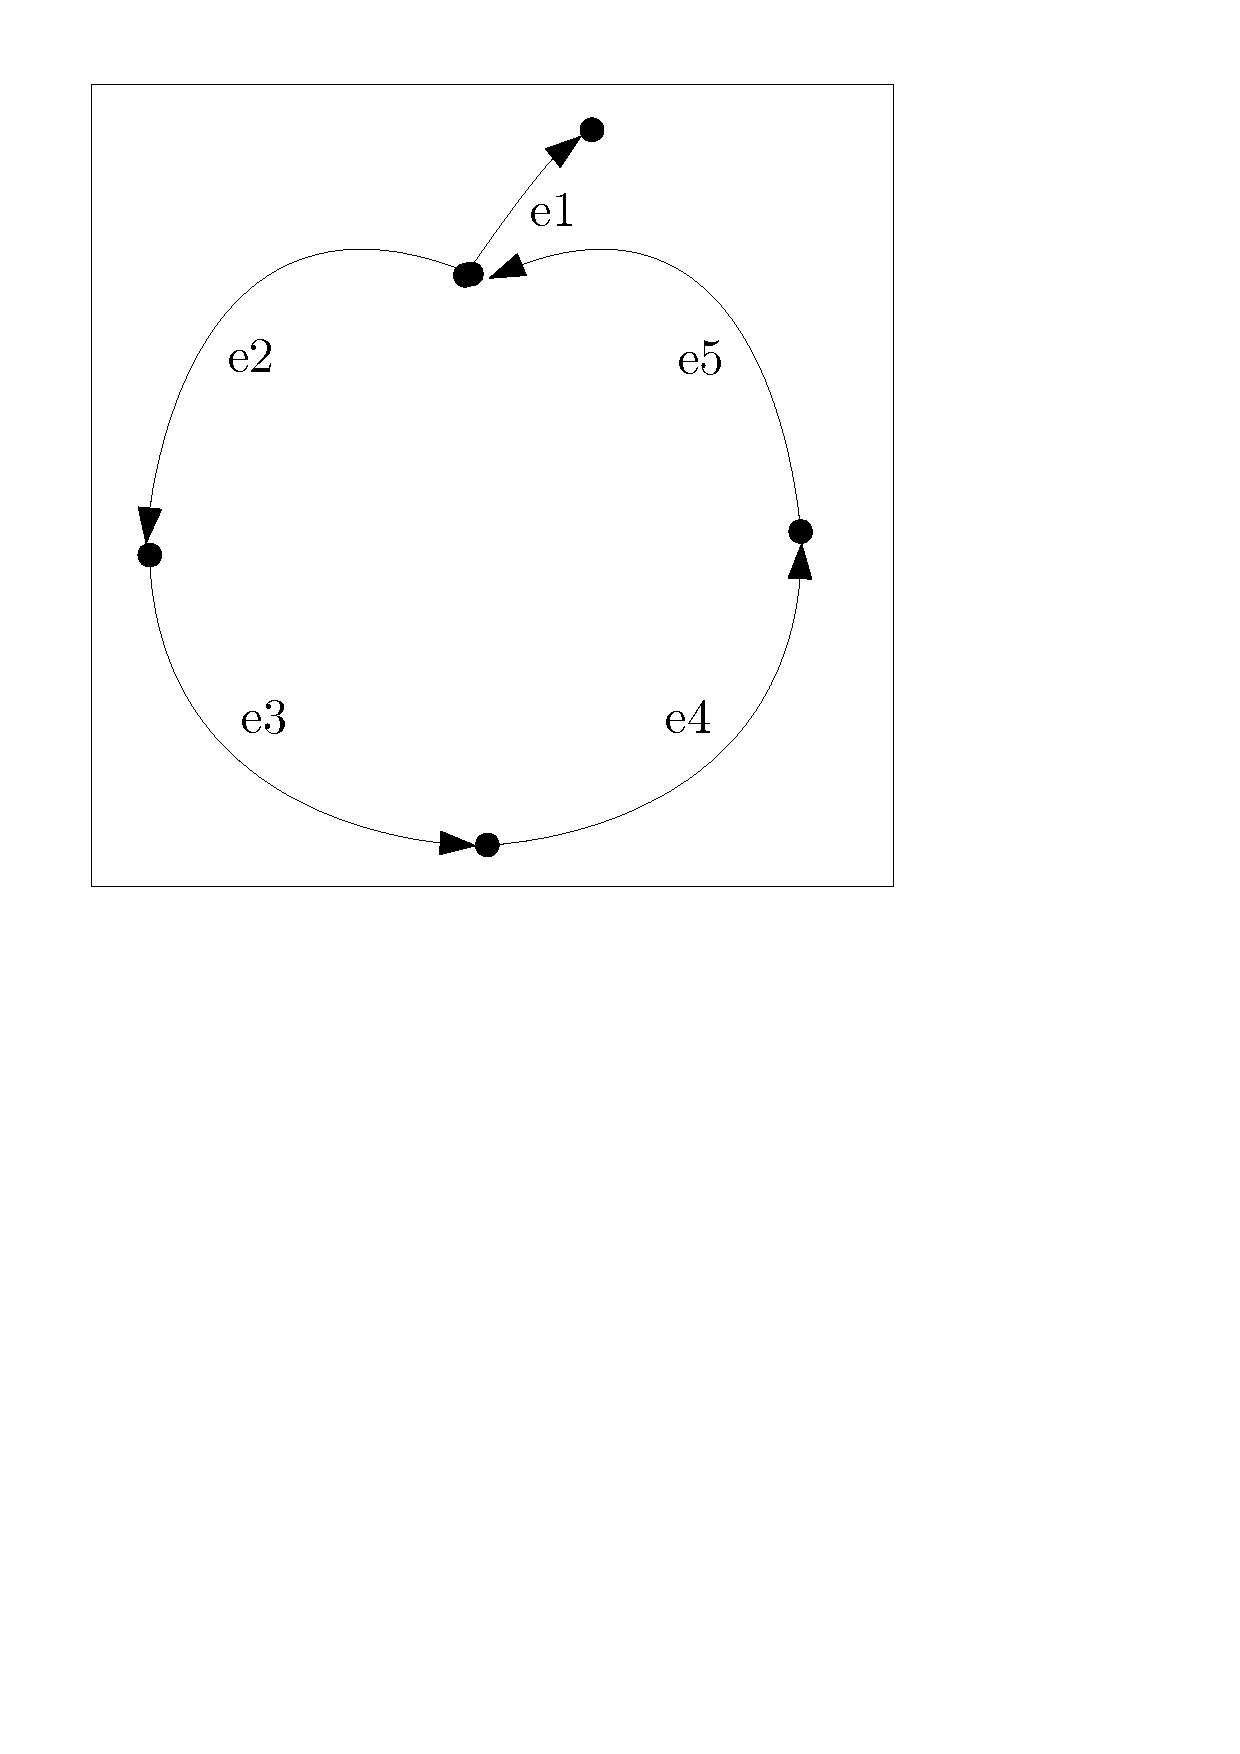
\includegraphics[width=3cm]{fig/apple} \end{array} \]
applied to $H$. We'll get the apple as new host graph $H'$. Now we want to rewrite our apple with stem to an apple with a leaflet. We use
\[ p':  \begin{array}[c]{c} 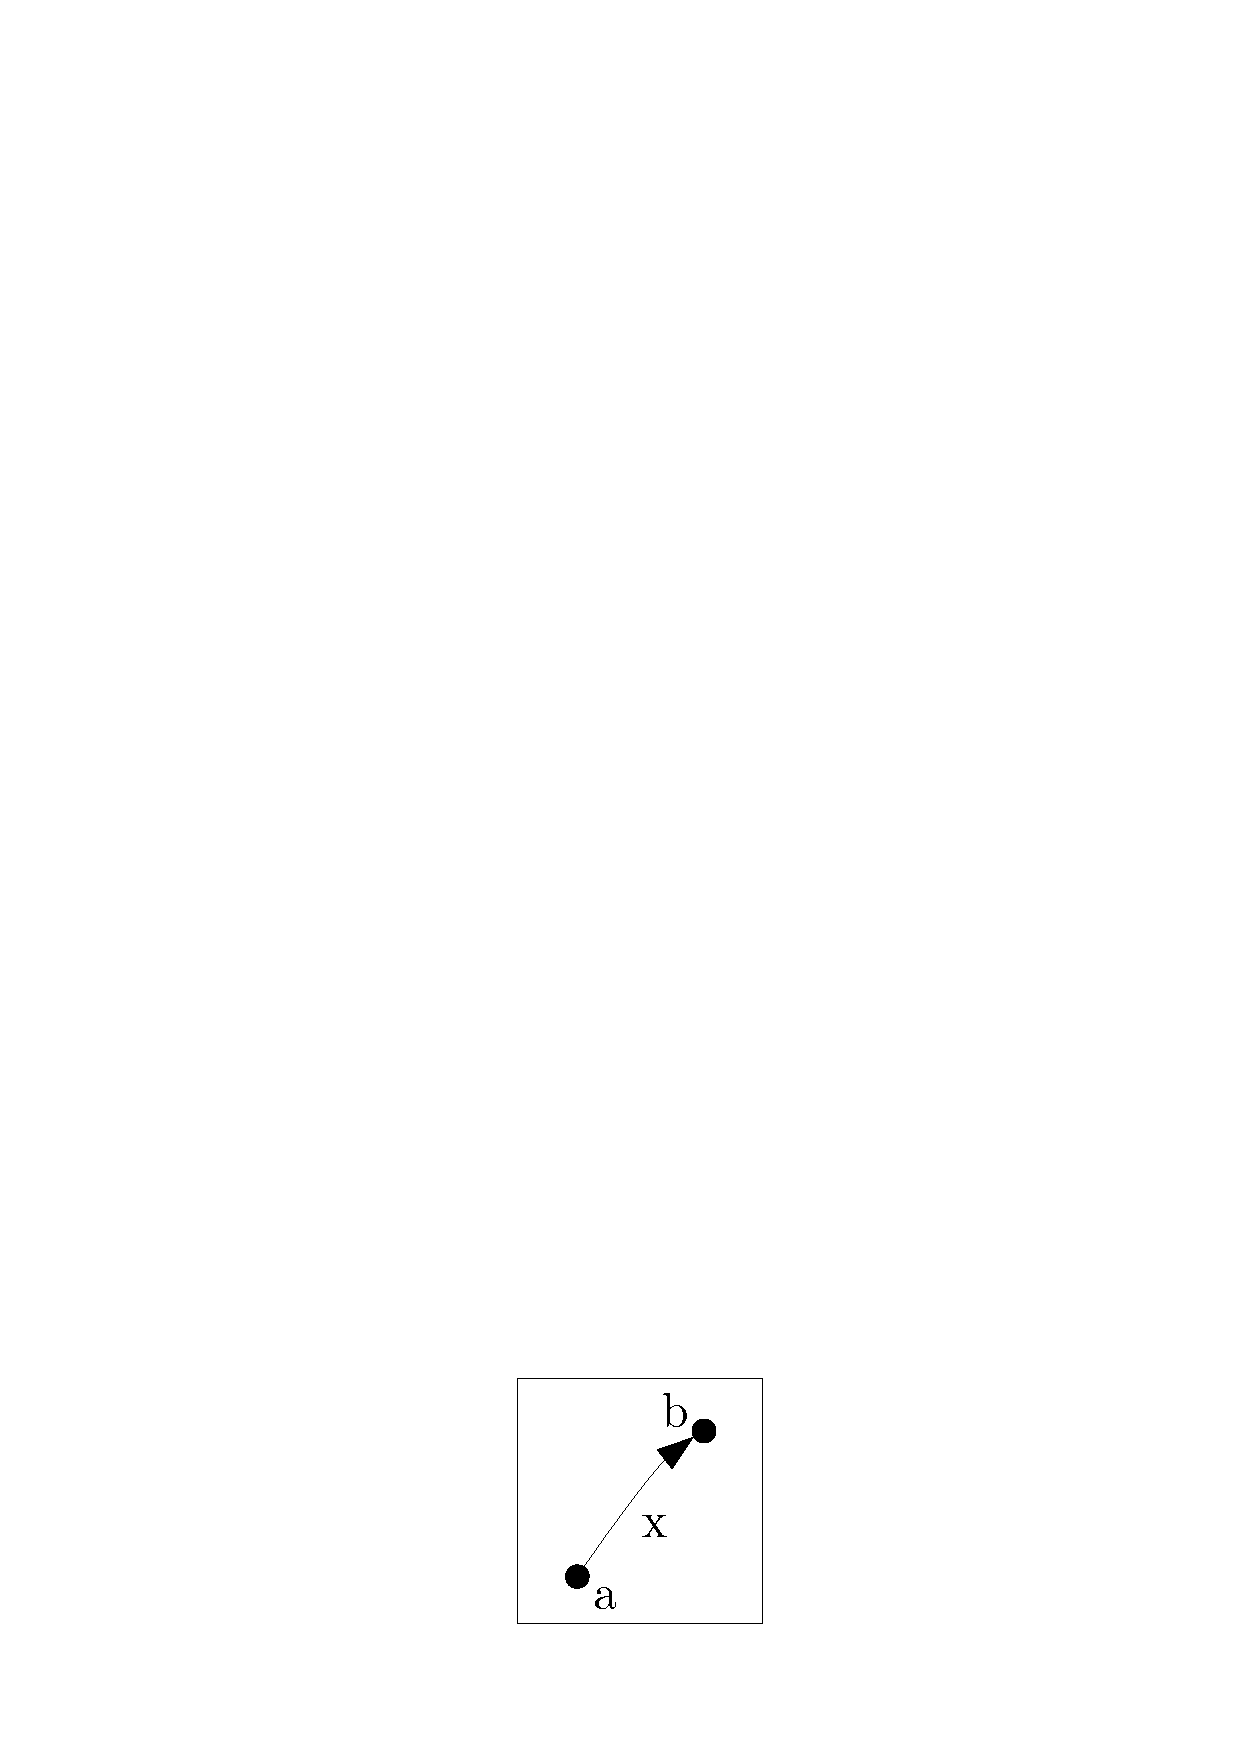
\includegraphics[height=1.25cm]{fig/stiel} \end{array} \begin{array}[c]{c} \longrightarrow \end{array} \begin{array}[c]{c} 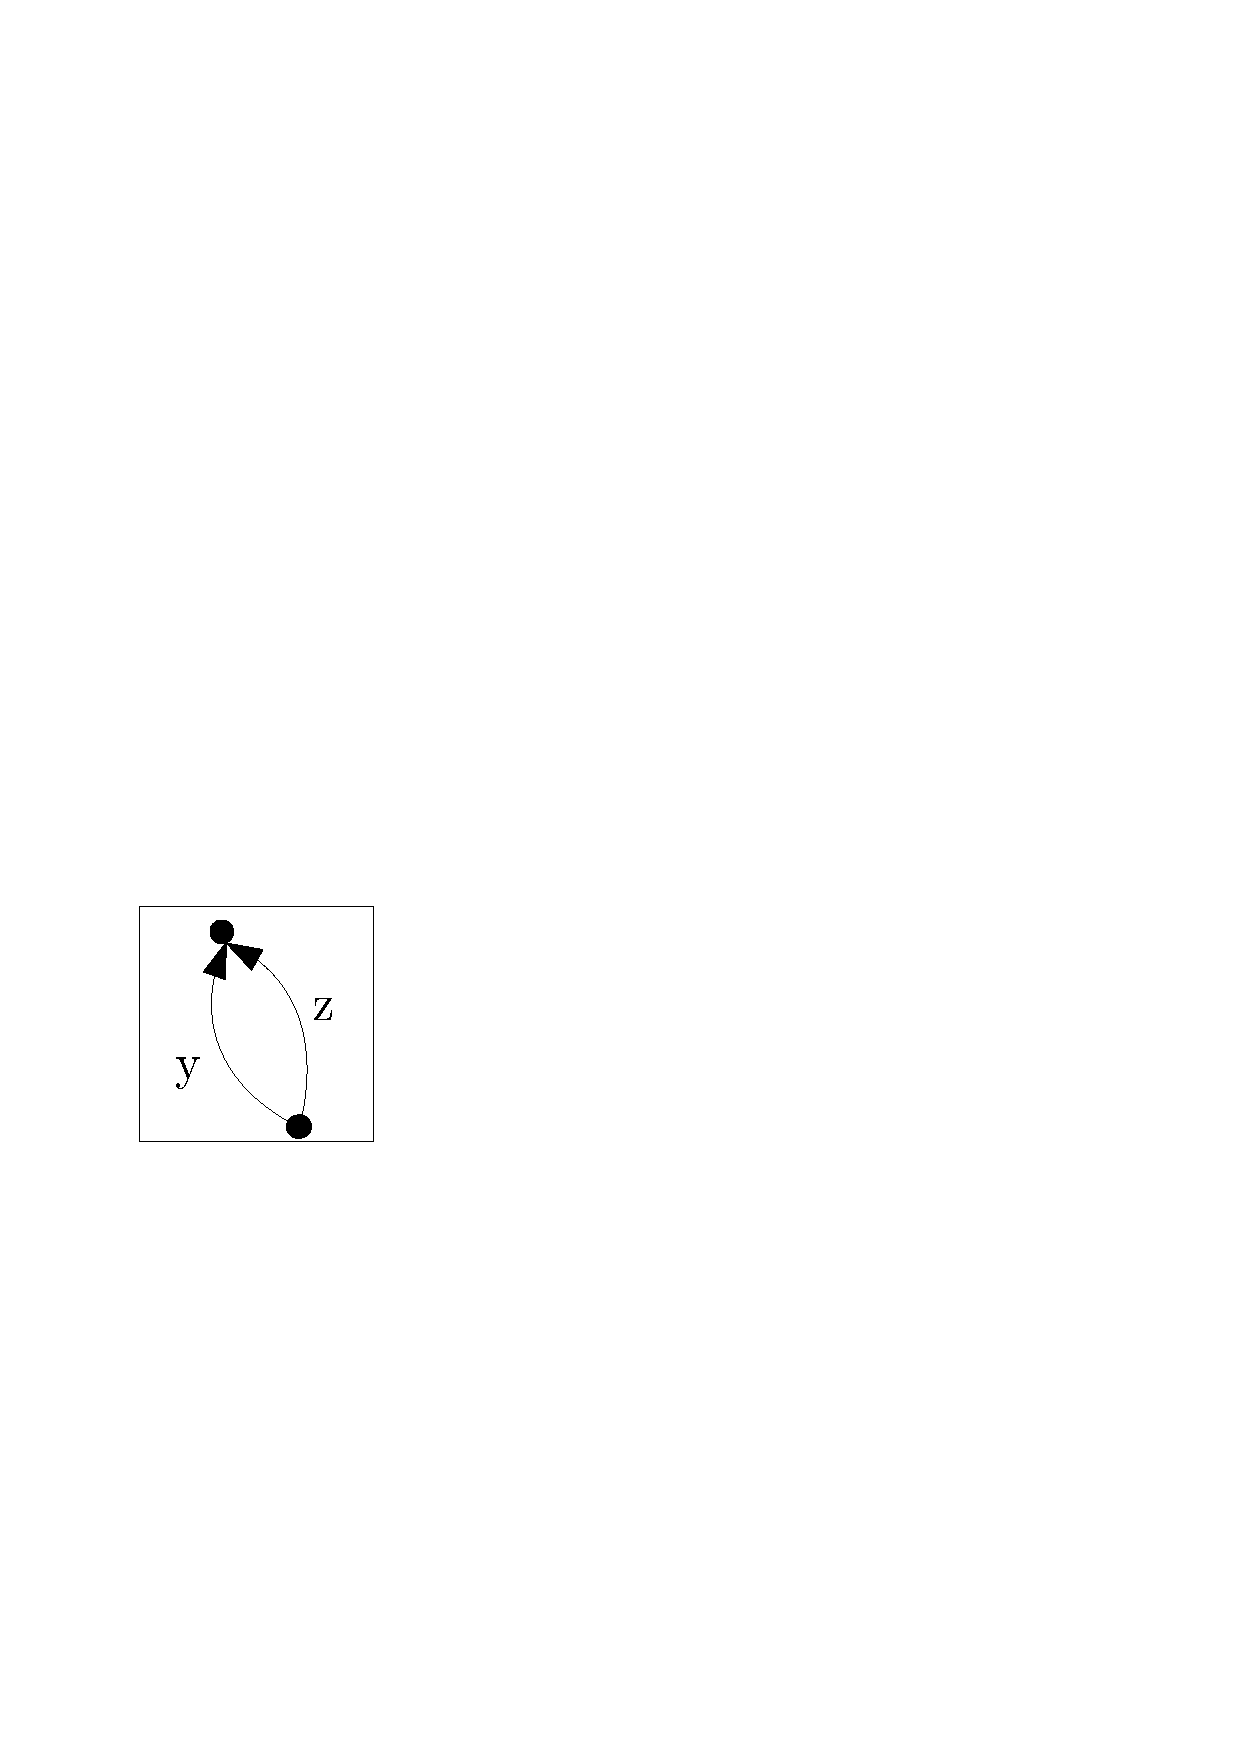
\includegraphics[height=1.25cm]{fig/blatt} \end{array}, \]
apply $p'$ to $H'$ and get the new host graph $H''$, something like this:
\[ 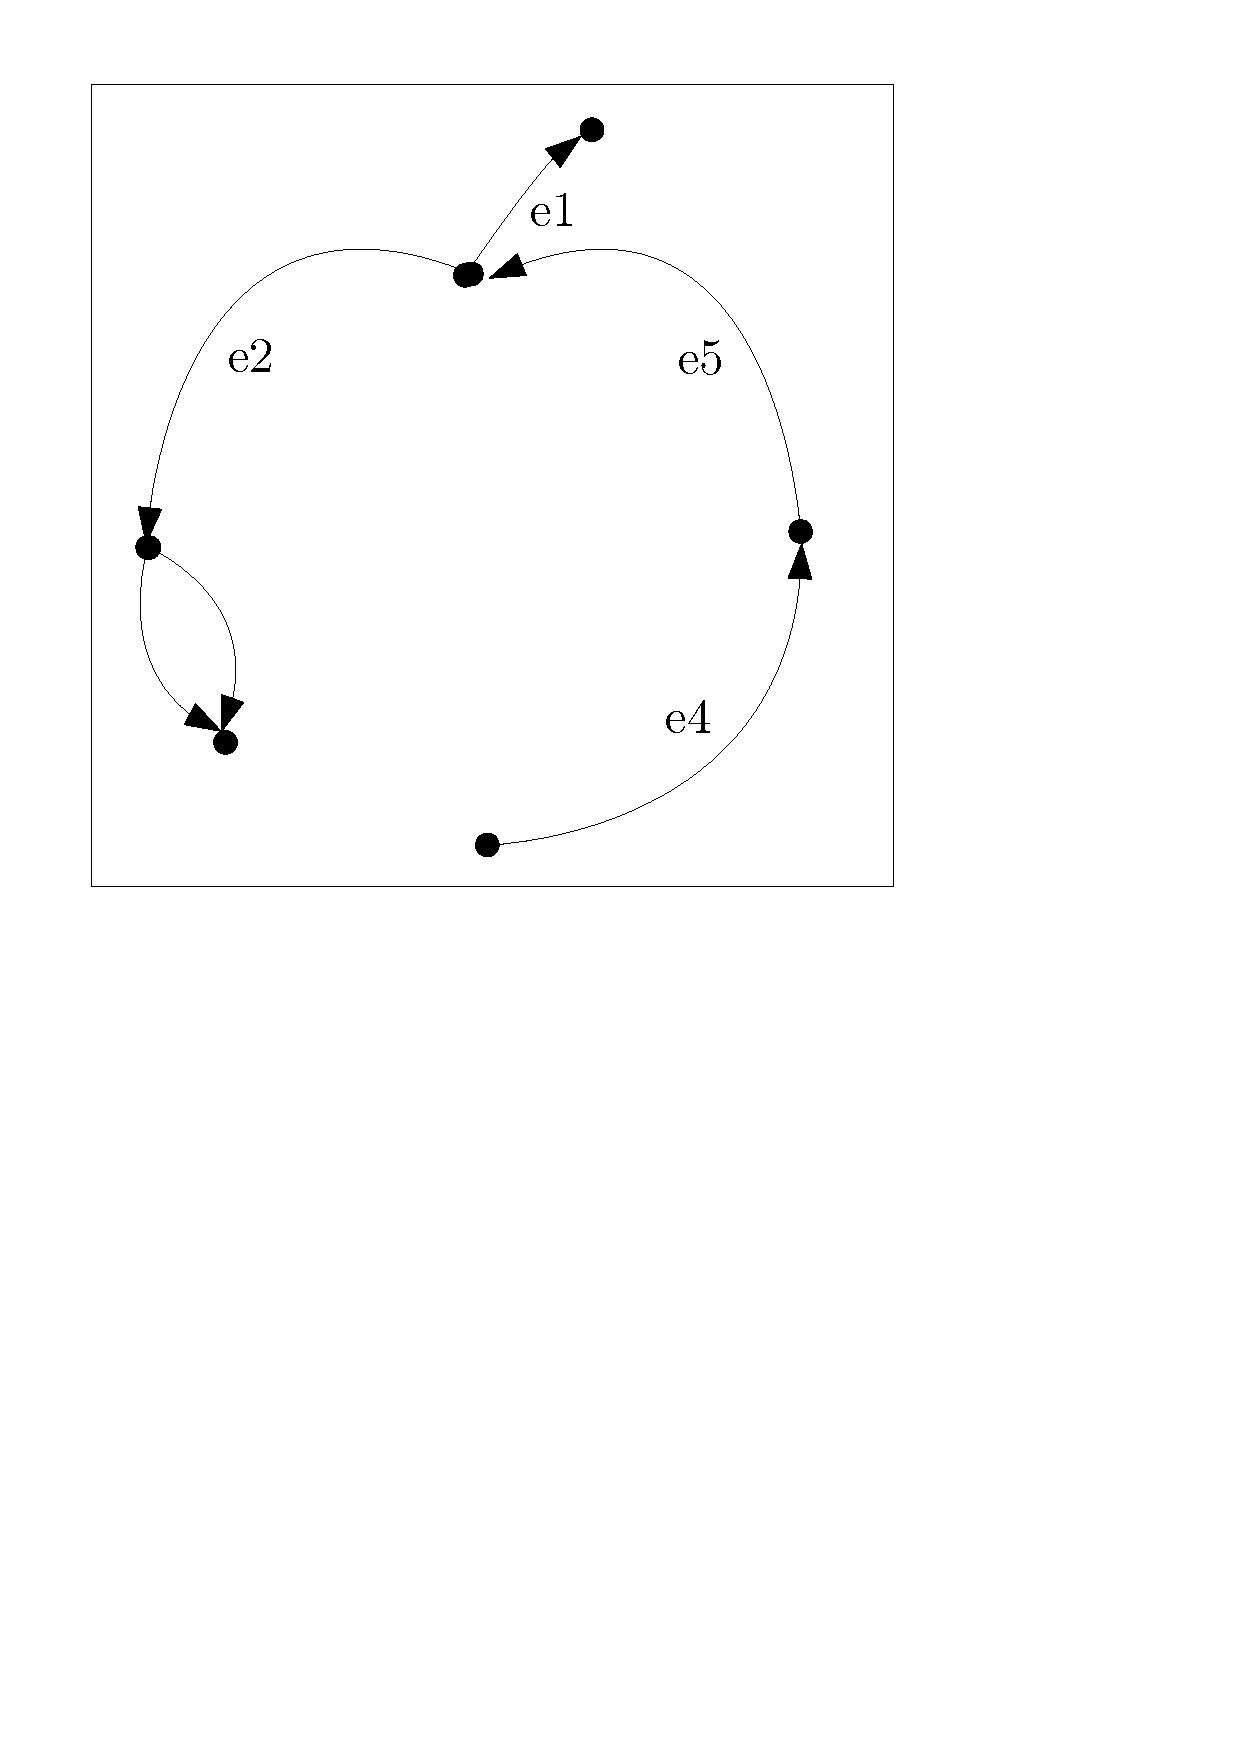
\includegraphics[width=3cm]{fig/wrongapple} \]
What happened? \GrG\ has randomly choosen a match, and $e3$ matches as well as $e1$. A correct solution could make use of edge type information. And this time we'll keep even the stem. So let $H''$ now be
\[ 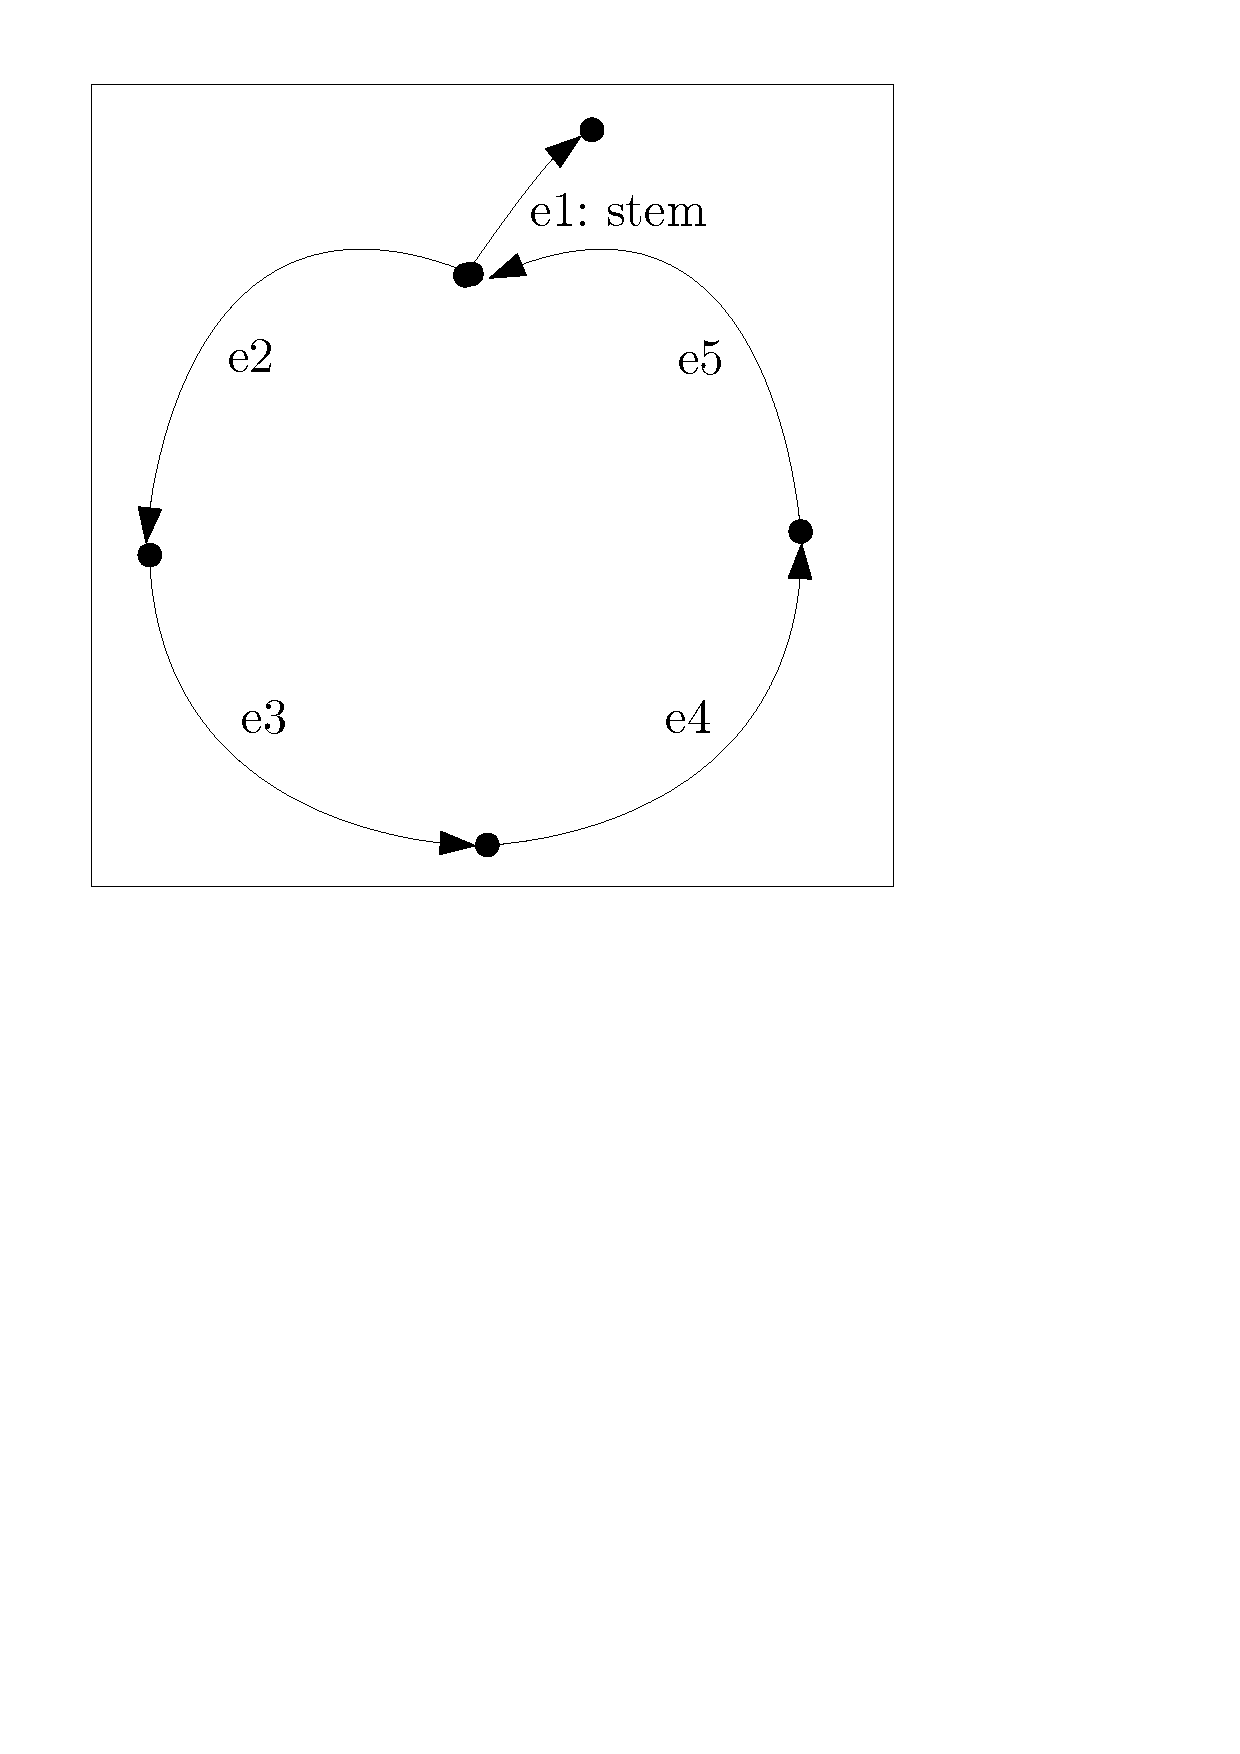
\includegraphics[width=3cm]{fig/typedapple} \]
and
\[ p'':  \begin{array}[c]{c} 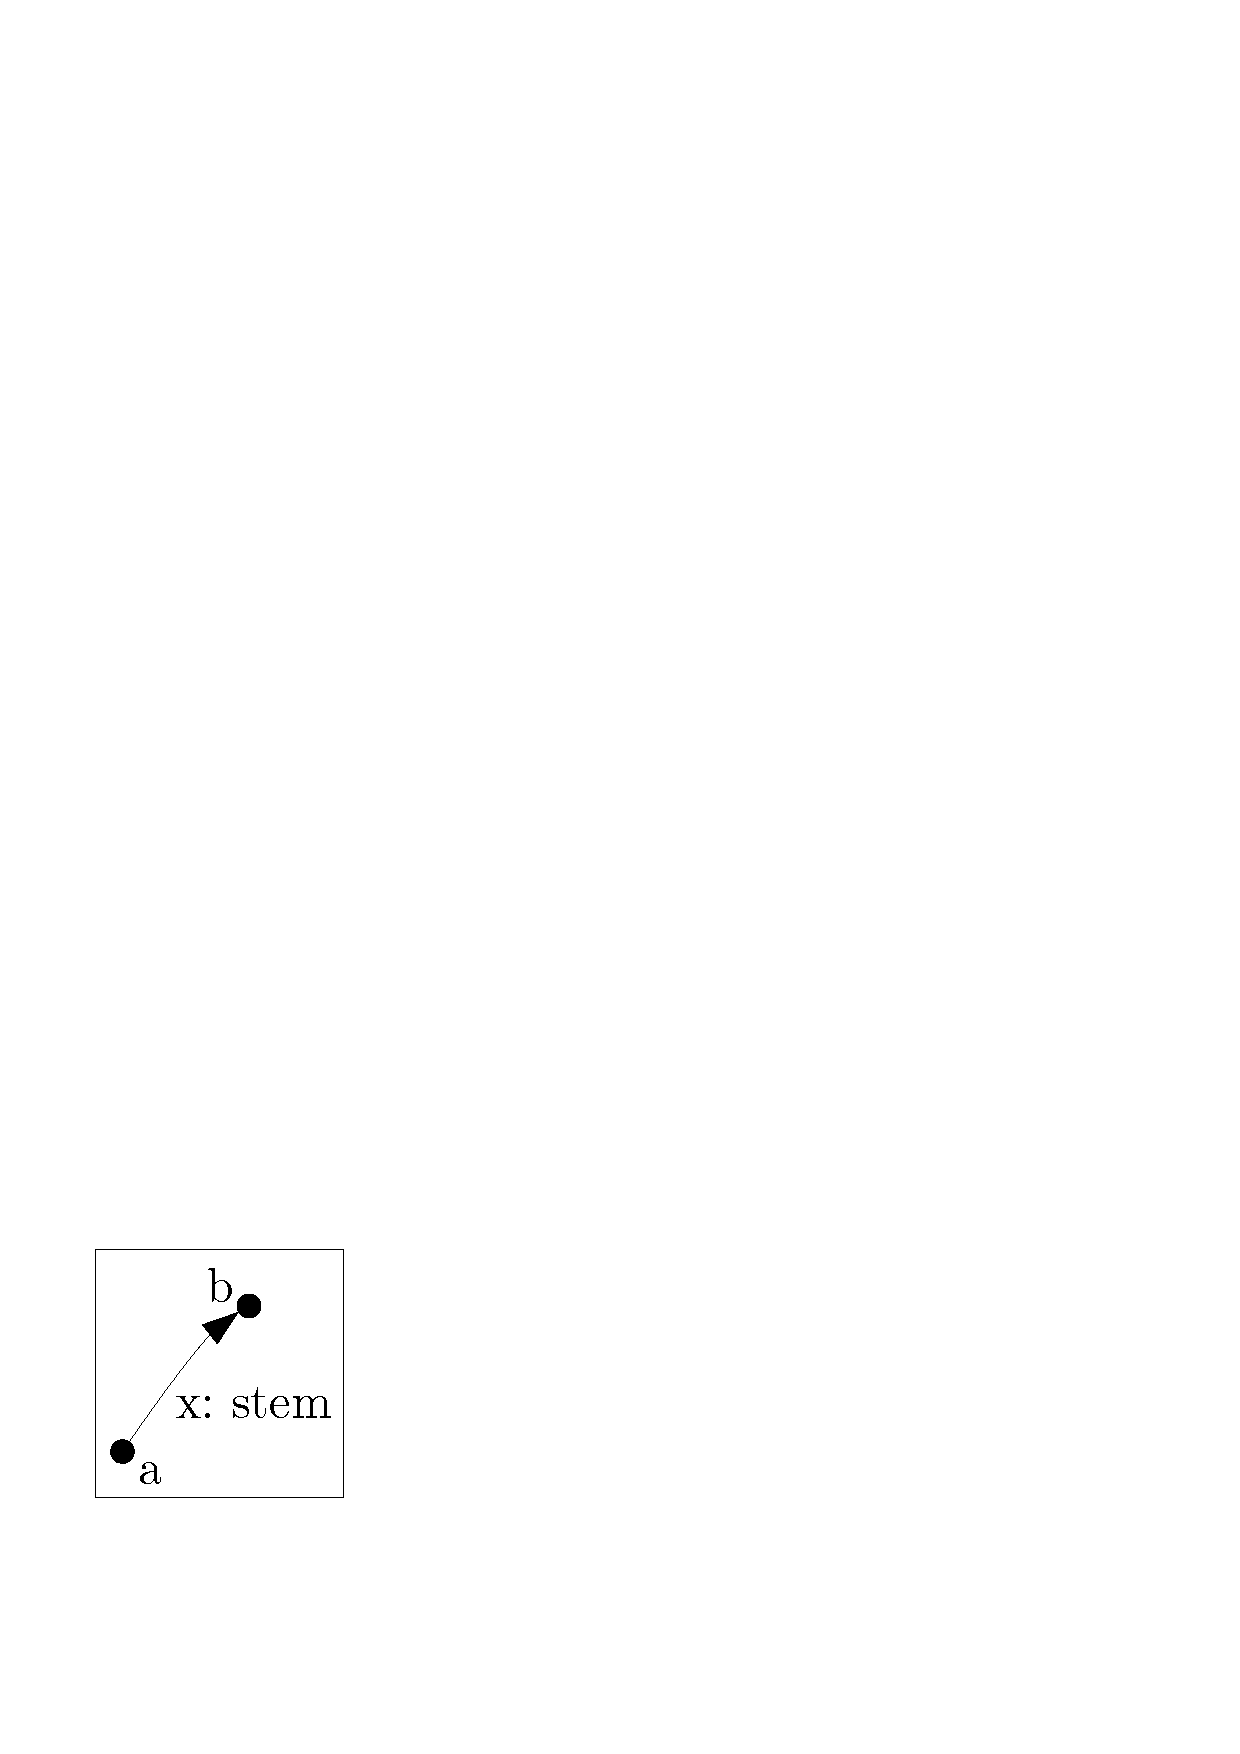
\includegraphics[height=1.25cm]{fig/typedstiel} \end{array} \begin{array}[c]{c} \longrightarrow \end{array} \begin{array}[c]{c} 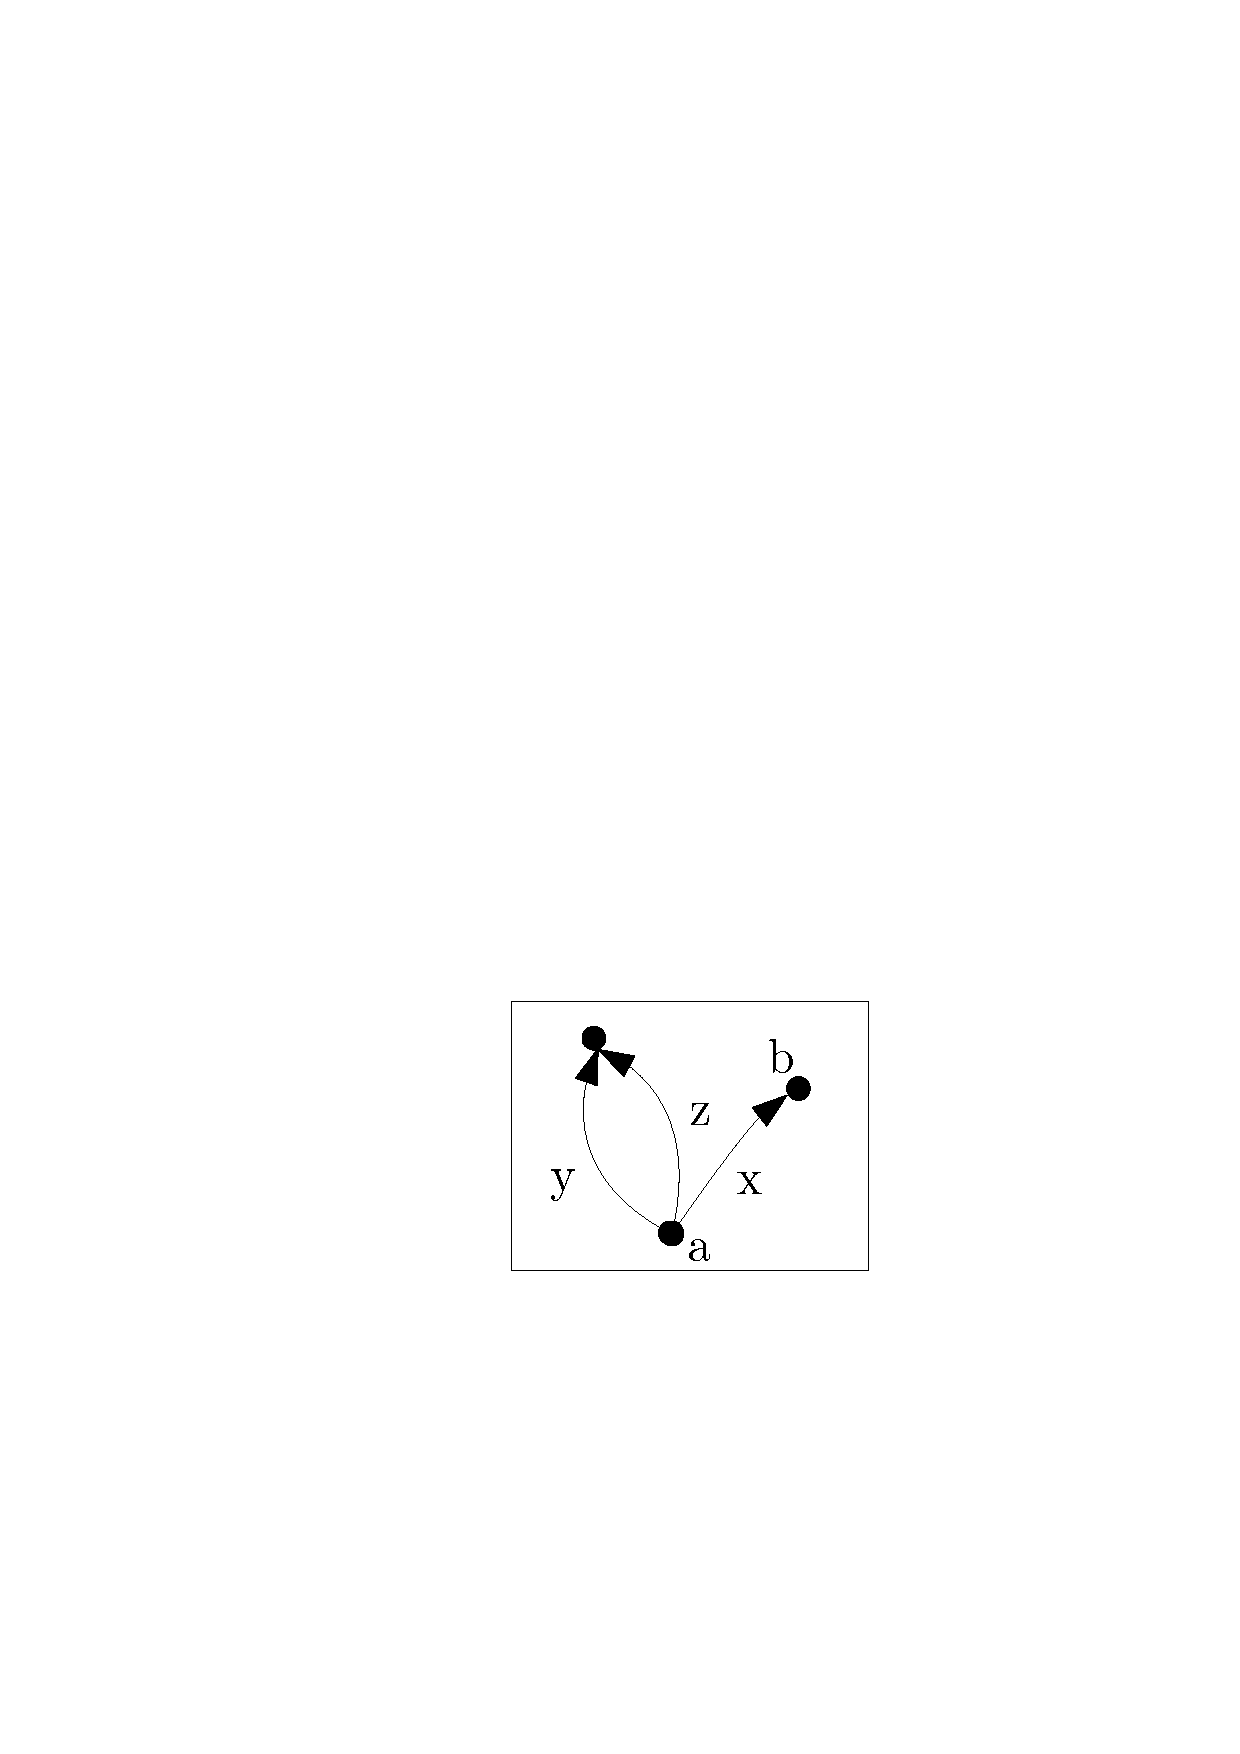
\includegraphics[height=1.25cm]{fig/typedblatt} \end{array}. \]
If we apply $p''$ to $H''$ this leads to
\[ 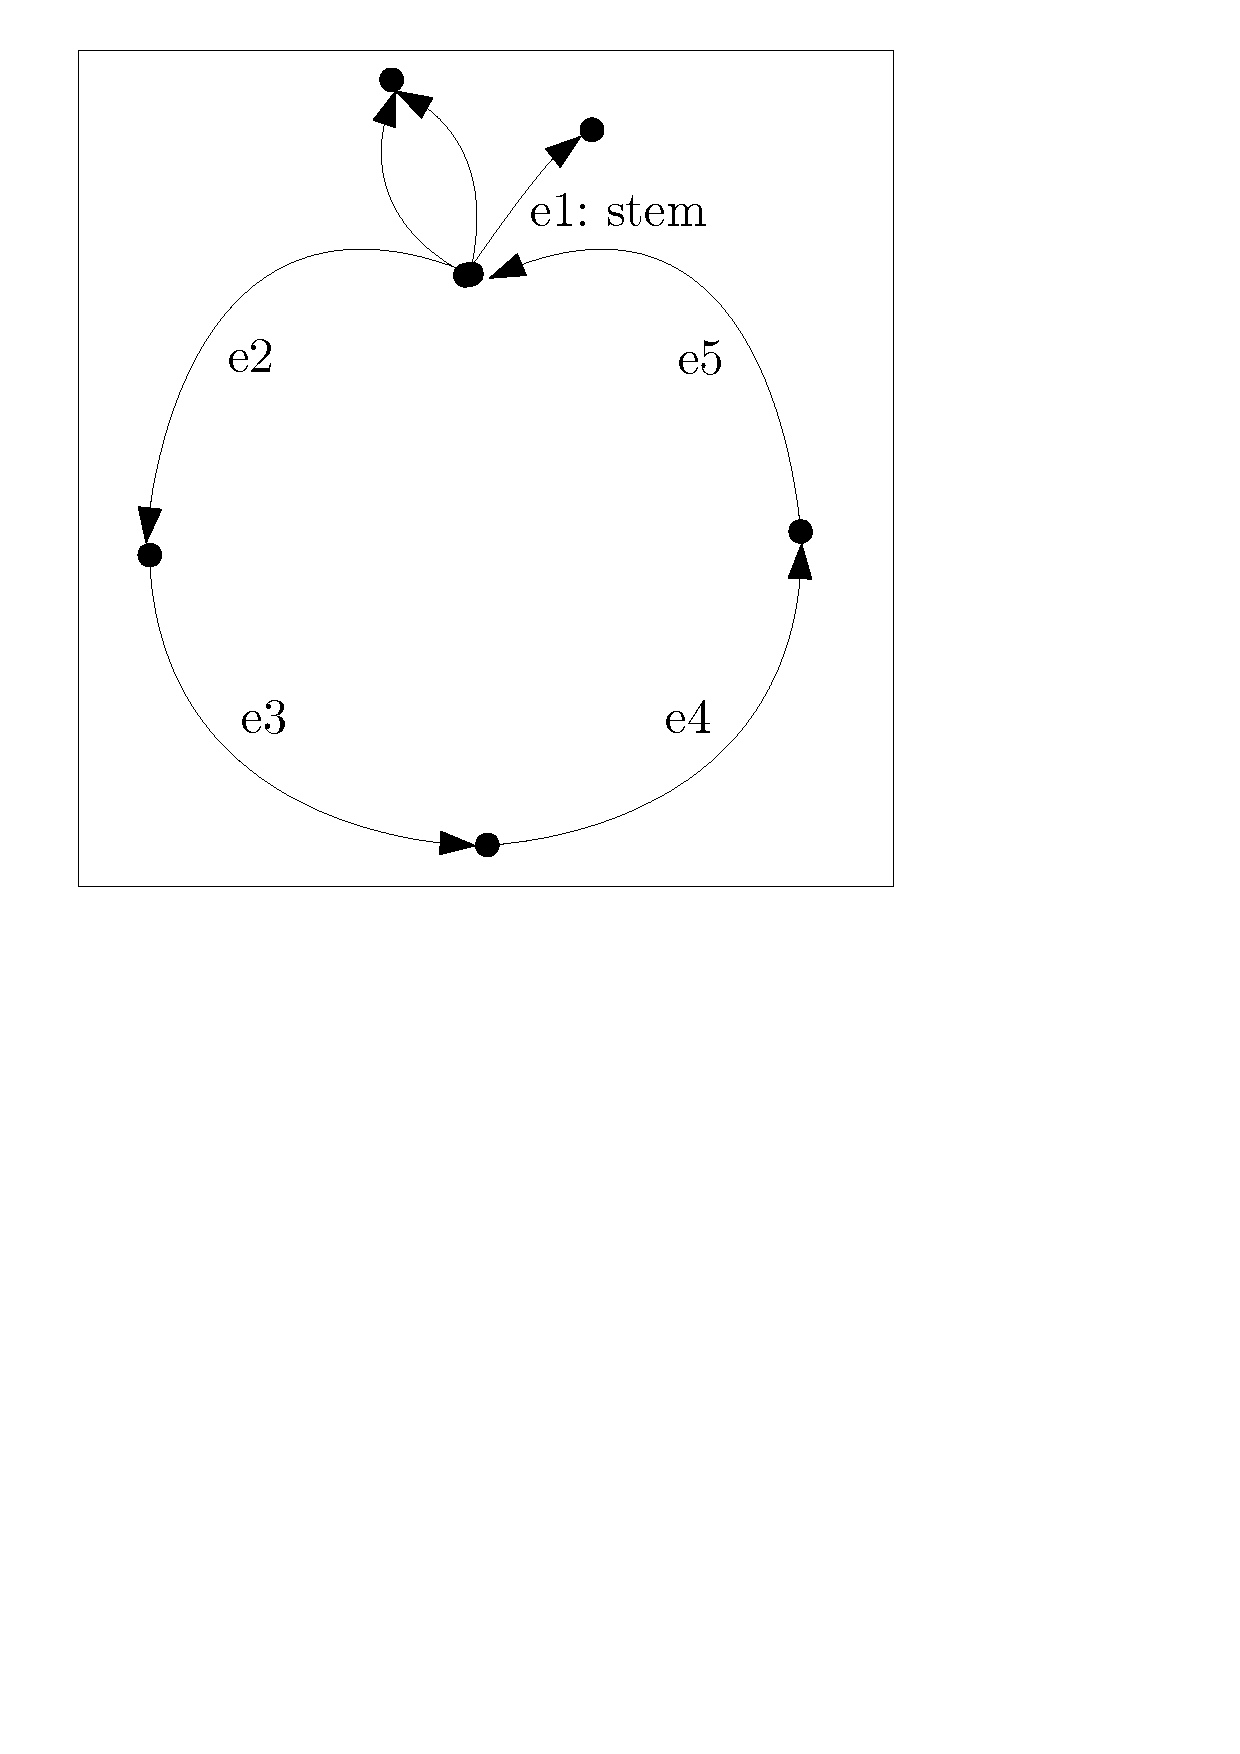
\includegraphics[width=3cm]{fig/rewrittenapple} \]
\emph{Note:} If we had applied $(p')*$ to $H'$ (execute $p'$ consecutively until no match is found) this would not have terminated, because each rewrite had produced one new canditate (one deleted, two added) for matching.    

\section{Components}
Figure \ref{figsys} gives an overview of the \GrG\ system components, whereas table \ref{dirstruc} shows the \GrG\ directory structure.
\begin{figure}[htbp]
  \centering
  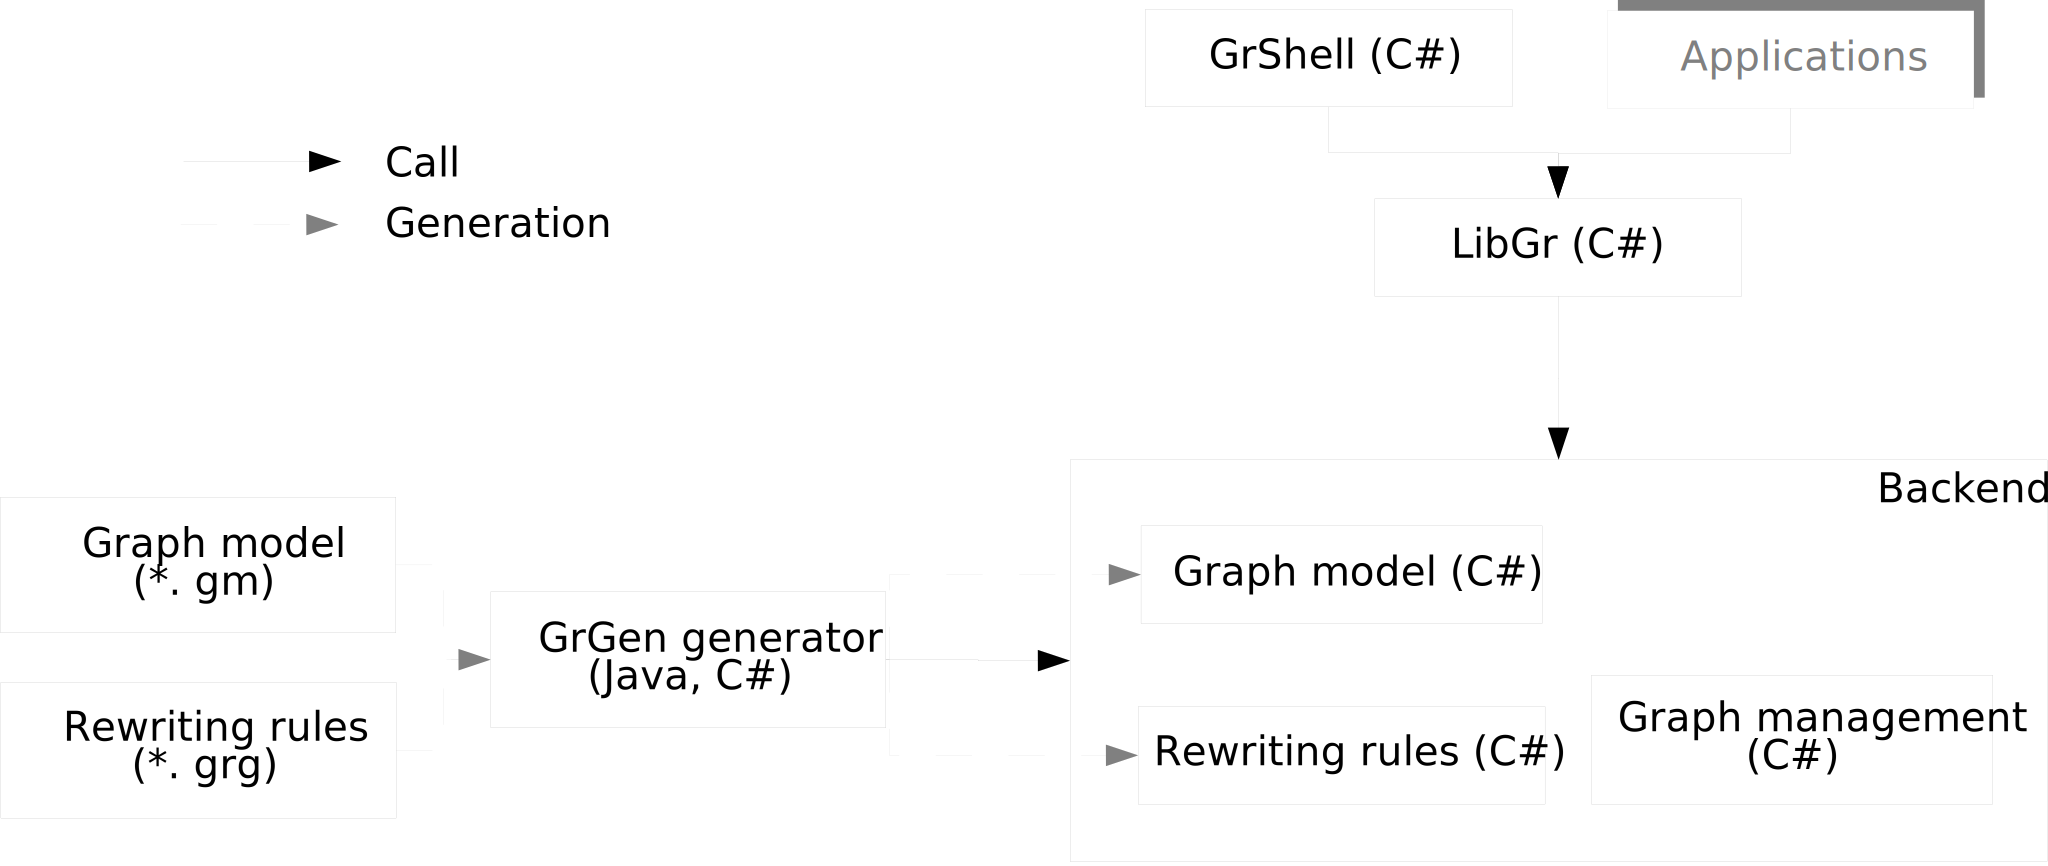
\includegraphics[width=\textwidth]{fig/Overview}
  \caption{\GrG\ system components \cite{kroll}}
  \label{figsys}
\end{figure}

\begin{table}[htbp]
  \begin{tabularx}{\linewidth}{|lX|} \hline
  bin & Contains the .NET assemblies, in particular GrGen.exe (the graph rewriting system generator), LGSPBackend.dll (a \GrG\ backend) and the shell GrShell.exe.  \\ 
  lib & Contains the \GrG\ generated assemblies (*.dll). \\
  specs & Contains the graph rewriting system source documents (*.gm and *.grg). \\ \hline
  \end{tabularx}
  \caption{\GrG\ directory structure}
  \label{dirstruc}
\end{table}

A graph rewriting system is defined by a rule set description file (*.grg) and one or more graph model description files (*.gm).\footnote{System, in this context, is not a CHO-like grammar rewriting system, but rather a set of interacting software components.} It is generated by GrGen.exe and can be used by \GrG\ applications such as GrShell. Figure \ref{process} shows the generation process.
\begin{figure}[htbp]
  \centering
  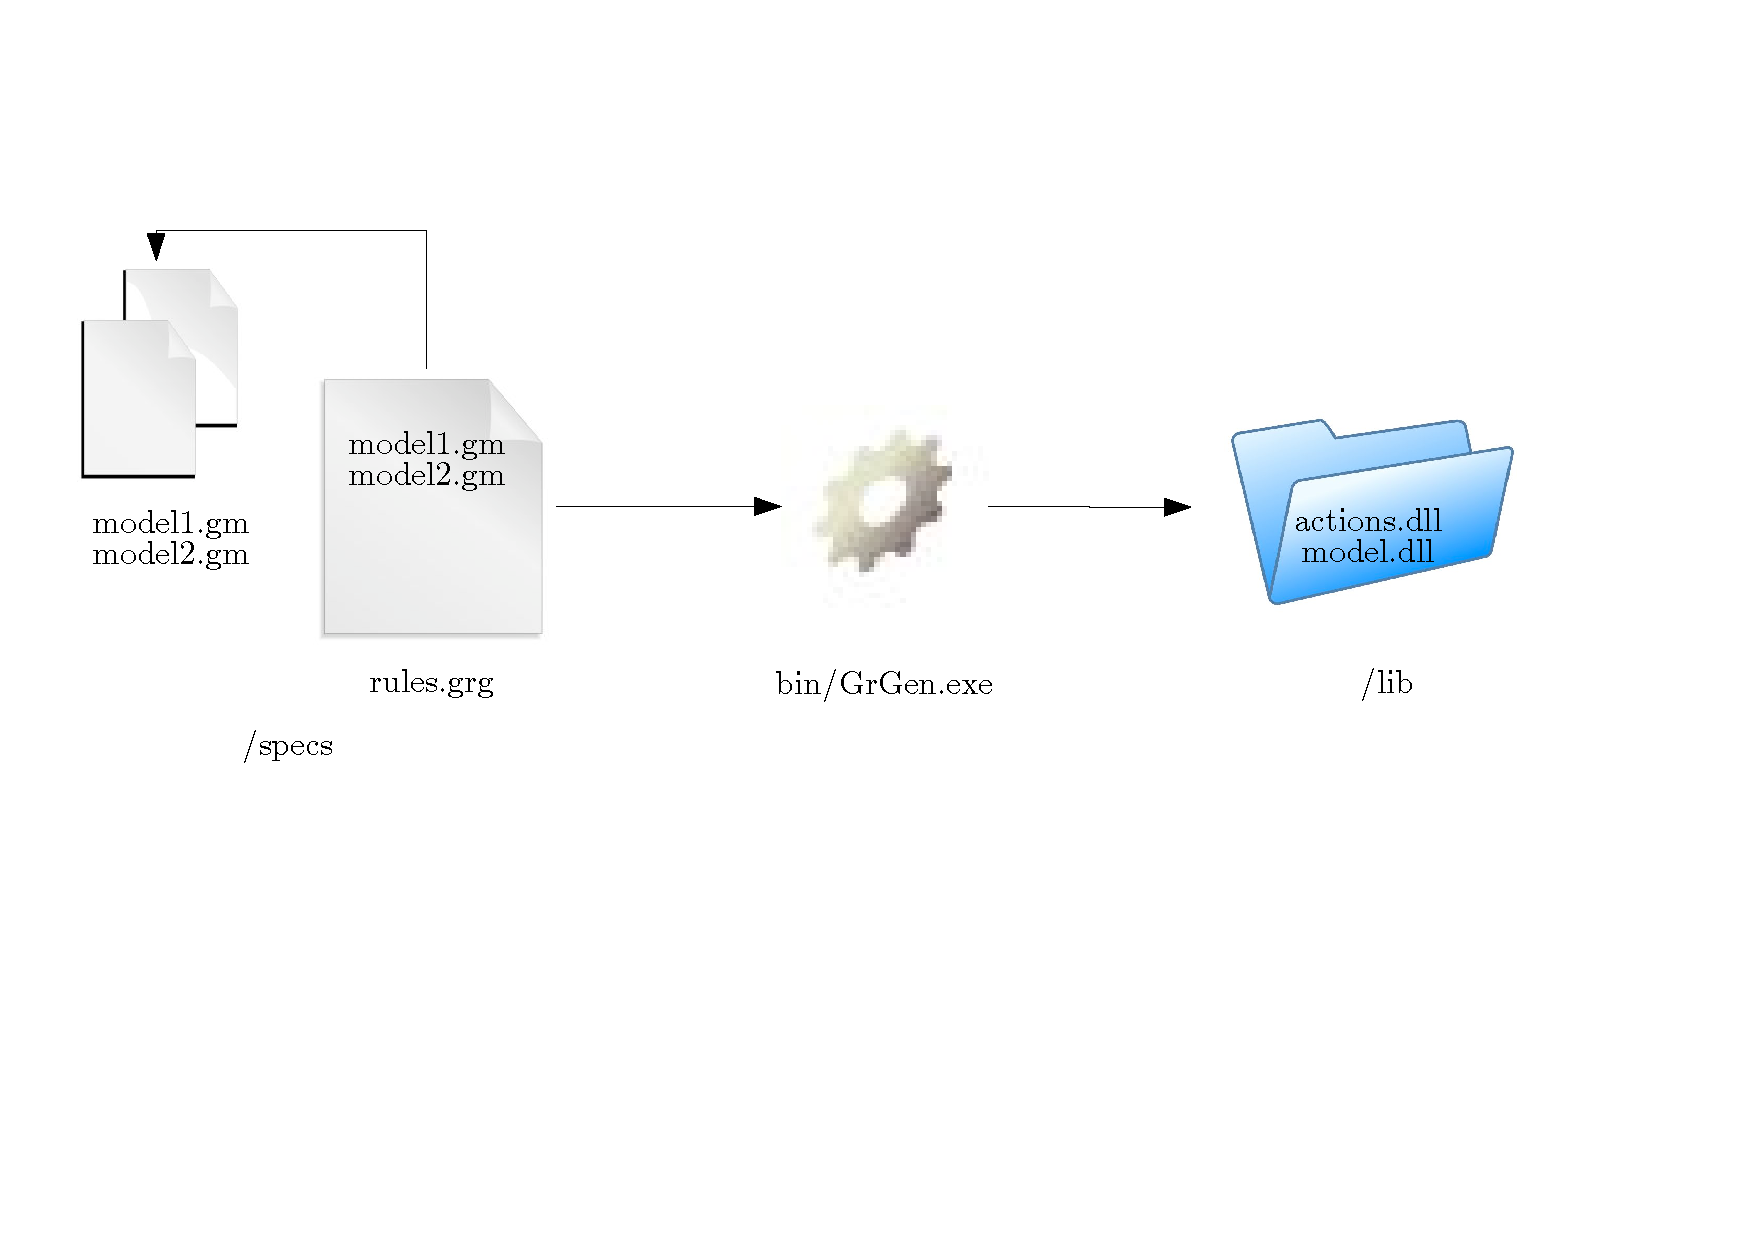
\includegraphics[width=\textwidth]{fig/process}
  \caption{Generating a graph rewriting system}
  \label{process}
\end{figure}

In general you have to distinguish carefully between a graph model (meta level), a host graph, a pattern graph and a rewriting rule. In \GrG\ pattern graphs are implicitly defined by rules, i.e.\ each rule defines its pattern. On the technical side, specification documents for a graph rewriting system can be available as source documents for graph models and rule sets (plain text *.gm and *.grg files) or as their translated .NET modules, either C\# source files or their compiled assemblies (*.dll).

\chapter{Graph Model Language}
The key features of \GrG\ graph models from \cite{geiss}:

\begin{description}
\item[Types.] Nodes and edges can have types (classes). This is similar to common programming languages, except \GrG\ types have no concept of methods. 
\item[Attributes.] Nodes and edges can possess attributes. The set of attributes assigned to a node or edge is determined by its type. The attributes itself are typed, too.
\item[Inheritance.] Types (classes) can be composed by multiple inheritance. \emph{Node} and \emph{Edge} are built-in root types of node and edge types, respectively. Inheritance eases the specification of attributes, because subtypes inherit the attributes of their super types. Note that \GrG\ lacks a concept of overwriting. On a path in the type hierarchy graph from a type up to the built-in root type there must be exactly one declaration for each attribute identifier.
\item[Connection Assertions.] To specify that certain edge types should only connect specific nodes, we include connection assertions. Furthermore the number of outgoing and incoming edges can be constrained.
\end{description}

\section{Basic Elements}

\emph{Note:} The following syntax specifications make heavy use of syntax diagrams (also known as rail diagrams). Syntax diagrams provide an visualization of EBNF grammars. Follow a path along the arrows from left to right through a diagram to get a valid sentence (or sub sentence) of the language. Ellipses are terminals whereas rectangles are non-terminals. For further information on syntax diagrams see \cite{

Basic elements of the \GrG\ graph model language are numbers and identifiers to denominate types, fields and the model itself. The \GrG\ graph model language is case sensitive.\\
\\
\emph{Ident}\\
A character sequence of arbitrary length consisting of letters, digits or underscores. The first character must not be a digit.\\
\\
\emph{NodeType}, \emph{EdgeType}, \emph{EnumType}\\
These are (semantic) specializations of Ident to restrict an identifier to a specific type.\\
\\
\emph{Number}\\
A sequence of digits. The sequence has to form a non-negative integer in decade system and will be internally stored in 32 bit tow's complement representation.

\section{Type Declarations}
\begin{rail}
  GraphModel: 'model' Ident ';' (() + TypeDeclaration);
\end{rail}
The graph model consists of its name \emph{Ident} and type declarations defining the type of nodes and edges.

\begin{rail}
  TypeDeclaration: EnumDeclaration | ClassDeclaration
\end{rail}
The primitive types \emph{int}, \emph{boolean} and \emph{string} are predefined. Types does not need to be declared before they are used.

\begin{rail}
  EnumDeclaration: 'enum' EnumType '(' ((Ident (() | '=' IntExpr)) + ',') ')' ';';
  ClassDeclaration: (() | 'abstract') (() | 'const') (NodeClass | EdgeClass);
  NodeClass: 'node' 'class' NodeType (() | 'extends' (NodeType+',')) \\ 
    (';' | lbrace FieldDeclarations rbrace);
  EdgeClass: 'edge' 'class' EdgeType (() | 'extends' (EdgeType+',')) \\
    (() + ConnectAssertions) (';' | lbrace FieldDeclarations rbrace);
  FieldDeclarations: (() | IdentDeclaration ':' FieldType ';') + ; 
  IdentDeclaration: Ident (() | '[' (Ident '=' Constant + ',') ']');
  FieldType: PrimitiveType | EnumType ; 
  ConnectAssertions: 'connect' (NodeConstraint '->' NodeConstraint + ',');
  NodeConstraint: NodeType (() | '[' ('*' | '+' | Number | RangeConstraint) ']') ;
  RangeConstraint: Number ':' ('*' | Number) ;
\end{rail}

\section{Expressions}
\label{expressions}

\begin{rail}
  Expression: BooleanExpr | IntegerExpr | PrimaryExpr;
  BooleanExpr: ((() | '(' 'boolean' ')') (() | '!') PrimaryExpr) | (BooleanExpr '?' BooleanExpr ':' BooleanExpr) | (BooleanExpr ([1] doubleampersand | [2] '||') BooleanExpr) | (Expression CompareOperator Expression);
  IntegerExpr: ((() | '(' 'int' ')') (() | '+' | '-' | tilde) PrimaryExpr) | (BooleanExpr '?' IntegerExpr ':' IntegerExpr) | (IntegerExpr BinaryOperator IntegerExpr);
  PrimaryExpr: '(' Expression ')' | Identifier (() | ('.' Identifier +)) | (EnumType '::' Identifier) | Constant;
  Constant: Number | HexNumber | QuotedText | 'true' | 'false';
\end{rail}

\emph{CompareOperator} is one of the following operators:
\[ \texttt{<} \;\;\;\;\; \texttt{<=} \;\;\;\;\; \texttt{==} \;\;\;\;\; \texttt{!=} \;\;\;\;\; \texttt{>=} \;\;\;\;\; \texttt{>} \]
\emph{BinaryOperator} is one of the operators in table \ref{tabbinops}:
\begin{table}[htbp] 
  \centering
  %\begin{tabularx}{0.45\linewidth}{|ll|} \hline
  \begin{tabular}[c]{|lp{0.5\linewidth}|} \hline
    \begin{tabular}[c]{l} \texttt{|} \\ \texttt{\^} \\ \texttt{\&} \end{tabular} & \begin{tabular}[c]{l} Binary OR, XOR and binary AND \end{tabular} \\ \hline
    \begin{tabular}[c]{l} \texttt{\mbox{<}\mbox{<}} \\ \texttt{\mbox{>}\mbox{>}} \\ \texttt{\mbox{>}\mbox{>}\mbox{>}} \end{tabular} & \begin{tabular}[c]{l} Bitwise shift left, bitwise shift right and \\ bitwise shift right with respect to sign \end{tabular}\\ \hline
    \begin{tabular}[c]{l} \texttt{+} \\ \texttt{-} \end{tabular} & \begin{tabular}[c]{l} Addition and subtraction \end{tabular}\\ \hline
    \begin{tabular}[c]{l} \texttt{*} \\ \texttt{/} \\ \texttt{\%} \end{tabular} & \begin{tabular}[c]{l}Multiplication, integer division \\ and modulo \end{tabular} \\ \hline
  \end{tabular}
  \caption{Binary integer operators, in ascending order of precedence}
  \label{tabbinops}
\end{table}  
MODULO, 32BIT 2erkomplement??

\chapter{Rule Set Language}

\section{Basic Elements}
TypeName, NodeType, EdgeType, Identifier, RuleSetName

\begin{rail}
  'actions' RuleSetName 'using' ((ModelName)+',') ';' \\ ((TestDeclaration | RuleDeclaration)+) ;
\end{rail}
In case of multiple graph models beware of conflicting declarations.

\begin{rail}
  ForwardEdge: '-' EdgeRefinement '->' ;
  ReverseEdge: '<-' EdgeRefinement '-' ;  
  EdgeRefinement: () | Identifier | ':' EdgeType | Identifier ':' EdgeType (() | TypeConstraint) ;
\end{rail}

\section{Declarations}
\begin{rail}
  TestDeclaration: 'test' ActionSignature lbrace Pattern rbrace ;
  RuleDeclaration: 'rule' ActionSignature lbrace Pattern Replace (() | Evaluation) rbrace ;
  ActionSignature: ActionName (() | Parameters) (() | ':' ReturnTypes) ;
  Parameters: '(' (() | (('node' Identifier ':' NodeType | 'edge' Identifier ':' EdgeType) + ',')) ')' ;
  ReturnTypes: '(' (() | (TypeName + ',') ) ')' ;
\end{rail}

\section{Pattern Part}
\begin{rail}
  Pattern: 'pattern' lbrace (()+PatternStatement) rbrace ;
  PatternStatement: PatternConnections ';' |
    'node' (PatternNode+',') ';' |
    'negative' lbrace (()+PatternStatement) rbrace |
    'if' (BooleanExpr ';' | (lbrace (() | (BooleanExpr ';' +)) rbrace)) |
    'return' '(' (Identifier+',') ')' ';' ;
\end{rail} 
An empty condition is true.

\begin{rail}   
  PatternConnections: (Identifier | PatternNode) (() | PatternContinuation) ;
  PatternNode: (Identifier ':' NodeType 
    | '(' (Identifier + ',') ')' ':' NodeType
    | '(' Identifier (tilde Identifier+) ')' ':' NodeType ) \\
      (() | TypeConstraint) ; 
  PatternContinuation: (ForwardEdge | ReverseEdge) (Identifier | PatternNode) (() | PatternContinuation) |
    '(' (PatternContinuation+',') ')' ; 
\end{rail}

\section{Replace Part}
\emph{Note:} Although \GrG\ does -- in general -- graph re\emph{writing} (also called graph transformation) this part has a re\emph{place} semantics.
\begin{rail}
  Replace: 'replace' lbrace (()+ReplaceStatement) rbrace ;
  ReplaceStatement: (ReplaceConnections |
    'node' (ReplaceNode+';') | 
    'return' '(' (Identifier+',') ')' ) ';' ;
  ReplaceConnections: (Identifier | ReplaceNode) (() | ReplaceContinuation) ;
  ReplaceNode: Identifier ':' NodeType (() | '<' Identifier '>') 
    | '(' (Identifier+',') ')' ':' NodeType ;
  ReplaceContinuation:  (ForwardEdge | ReverseEdge) (Identifier | ReplaceNode) (() | ReplaceContinuation) |
    '(' (ReplaceContinuation+',') ')' ;    
\end{rail}
REPLACE??

\section{Evaluation Part}
\begin{rail}
  Evaluation: 'eval' lbrace (() + Assignment) rbrace ;
  Assignment: Identifier ('.' Identifier +) '=' Expression ';'
\end{rail} 

\section{Type Expressions}
\begin{rail}
  TypeConstraint: backslash '(' TypeExpression ')' ;   
  TypeExpression: PrimaryTypeExpr | TypeExpression ([1] '+' | [2] backslash | [3] ampersand) TypeExpression ;
  PrimaryTypeExpression: ':' TypeName | lbrace (TypeName+',') rbrace | '(' TypeExpression ')';
\end{rail}
Table \ref{tabtypeops} explains the type expression operators in order of precedence, starting with the least precedence.
\begin{table}[htbp]
  \centering
  \begin{tabular}{|ll|} \hline
    \texttt{+} & bla\\
    \texttt{\char"5C} & bla\\
    \texttt{\&} & bla \\ \hline
  \end{tabular}
  \caption{Type expression operators}
  \label{tabtypeops}
\end{table}  

\chapter{GrShell Language}

The GrShell is a shell application of the LibGr. It belongs to \GrG's standard equipment. GrShell is capable of creating, manipulating and dumping graphs as well as performing graph rewriting and debugging graph rewriting.

The GrShell language is a line oriented scripting language. It is structured by simple statements separated by line breaks.

\section{Basic Elements}

The GrShell is case sensitive. A comment starts with a \emph{\#} and is terminated by end-of-line or end-of-file. Anything left from the \emph{\#} will be treated as a statement.

\begin{rail} 
 Text : '<DoubleQuotedText>' | '<SingleQuotedText>' | '<Word>' ;
 Number : '<Number>' ;
 TextOrNumber : Text | Number ;
 Parameters : Text + ',' ;
 SpacedParameters: Text + ; 
\end{rail}

Those items are required for representing text, numbers and parameters within rules. The tokens $<\cdots>$ are defined as follows:\\

\begin{tabularx}{\linewidth}{lX}
<Word>: & A character sequence consisting of letters, digits and underscores. The first character must not be a digit.\\
<DoubleQuotedText>: & Arbitrary text enclosed by double quotes (`` '').\\
<SingleQuotedText>: & Arbitrary text enclosed by single quotes (` ').\\
<Number>: & A sequence of digits.
\end{tabularx}\\

In order to describe the possible input to some of the commands more precisely, the following (semantic) specializations of \emph{Text} are defined:\\

\begin{tabularx}{\linewidth}{lX}
Filename: & A file path without spaces (e.g.\ /Users/Bob/amazing\textunderscore file.txt) or a single quoted or double quoted file path that may contain spaces (``/Users/Bob/amazing\textunderscore file.txt'').\\
Variable: & Identifier of a variable that contains a graph element.\\
NodeType: & Identifier of a node type within the model of the current graph.\\
AttributeName: & Identifier of an attribute.\\
Graph: & Identifies a graph by its name. \\
Action: & Identifies a rule by its name.\\
Color: & One of the following color identifiers: Black, Blue, Green, Cyan, Red, Purple, Brown, Grey, LightGrey, LightBlue, LightGreen, LightCyan, LightRed, LightPurple, Yelloq, White, DarkBlue, DarkRed, DarkGreen, DarkYellow, DarkMagenta, DarkCyan, Gold, Lilac, Turquoise, Aquamarine, Khaki, Pink, Orange, Orchid.
\end{tabularx}\\

The elements of a graph (nodes and edges) can be accessed both by their variable identifier and by their persistent name specified through a constructor (see \ref{mani}):
\makeatletter
\begin{rail}
  GraphElement: Text | ('@' '(' Text ')')
\end{rail}
\makeatother
The specializations \emph{Node} and \emph{Edge} of \emph{GraphElement} requires the corresponding graph element to be a node or an edge respectively.\\

%\lined 
{\label{persistentex} \small \textbf{Example:} We insert a node, anonymously and with a constructor:
\lstset{language=grshell}
\begin{lstlisting}
> new graph "../lib/lgsp-TuringModel.dll" G
New graph "G" of model "Turing" created.
  
# insert an anonymous node... 
# it will get a persistent pseudo name
> new :State  
New node "$0" of type "State" has been created.
> delete node @("$0")
  
# and now with constructor
> new v:State($=start) 
new node "start" of type "State" has been created.
# Variable v is now assigned to start
> new :State($=end)
new node "end" of type "State" has been created.
  
# actually we want v to be "end": 
>  v = @(end)
>
\end{lstlisting}}
%\lined
\emph{Note:} Persistent names belong to a specific graph, whereas variables belong to the current GrShell environment. Persistent names will be saved (\texttt{save graph\dots}) and, if you visualize a graph (\texttt{dump graph\dots}), graph elements will be labeled with their persistent names. Persistent names have to be unique for a graph. 

\begin{rail}
  Variable '=' GraphElement   
\end{rail}
Assigns the variable or persistent name \emph{GraphElement} to \emph{Variable}. If \emph{Variable} is not defined, it will be defined implicitly.

\section{GrShell Commands}
This section describes the GrShell commands. Commands are assembled from basic elements. As stated before commands are terminated by a line breaks. Alternatively commands can be terminated by the \texttt{;;} symbol.
\begin{rail}
  Script: ((Command ('<line break>' | ';;'))+) '<end of file>' ;
\end{rail}

\subsection{Common Commands}
\begin{rail}
  'help'
\end{rail}
Displays an information message describing supported commands. 

\begin{rail}
  'quit' | 'exit'
\end{rail}
Quits GrShell. If GrShell is opened in debug mode, currently active graph displayers (such as YComp) will be closed as well.

\begin{rail}
  'select' 'backend' Filename ( ( ) | ':' Parameters )
\end{rail}
Selects a backend that handles graph and rules representation. \emph{Filename} has to be a .NET assembly (e.g.\ ``lgspBackend.dll'').  Comma-separeted parameters can be supplied optionally. If so, the backend must support these parameters.

\begin{rail}
  'show' 'backend' Filename
\end{rail}
List all the parameters supported by the backend \emph{Filename}, that can be provided to the \texttt{select backend} command.

\begin{rail}
  'include' Filename
\end{rail}
Executes the GrShell script \emph{Filename}. A GrShell script is just a plain text file containing GrShell commands. They are treated as they would be entered interactively, except for parser errors. If an parser error occurs, execution of the script will cancel immediately.

\begin{rail}
  'debug' ( 'enable' | 'disable' )
\end{rail} 
Enables and disables the debug mode. The debug mode shows the current working graph in a YComp window. All changes to the working graph are tracked by YComp immediately.  

\begin{rail}
  'echo' Text
\end{rail}
Prints \emph{Text} onto the GrShell command prompt.

\subsection{Graph Commands}

\begin{rail}
  'new' 'graph' Filename Text 
\end{rail}
Creates a new graph with the model specified in \emph{Filename}. Its name is set to \emph{Text}. The model file can be either source code (e.g.\ ``turing\textunderscore machine.cs'') or a .NET assembly (e.g.\ ``turing\textunderscore machine.dll'').

\begin{rail}
  'open' 'graph' Filename Text
\end{rail}
Opens the graph \emph{Text} stored in the backend. Its model is specified in \emph{File\-name}. However, the \emph{LGSPBackend} doesn't support persistent graphs. \emph{LGSPBackend} is the only backend so far. Therefore this command is useless at the moment.

\begin{rail}
  'show' 'graphs'
\end{rail}
Displays a list of currently available graphs.

\begin{rail}
  'select' 'graph' Graph
\end{rail}
Selects the current working graph.

\begin{rail}
  'delete' 'graph' Graph
\end{rail}
Deletes the graph \emph{Graph} from the backend storage.

\begin{rail}
  'validate' ( ( ) | 'strict' )
\end{rail}
Validates if the current working graph fulfills the edge constraints specified in the corresponding graph model. The \emph{strict} mode additionally requires all the edges of the working graph to be specified in order to get a ``valid''. Otherwise edges between nodes without specified constraints are ignored.\\

{\small \textbf{Example:} We define a micro model of street map graphs:
\lstset{language=grgenmodel}
\begin{lstlisting} 
model Map;

node class city;
node class metropolis;

edge class street;
edge class highway
      connect metropolis [+] -> metropolis [+];
\end{lstlisting}
The node constraint on \emph{highway} requires all the metropolises to be connected by highways. Now have a look at the following graph:
\begin{center}
  \fbox{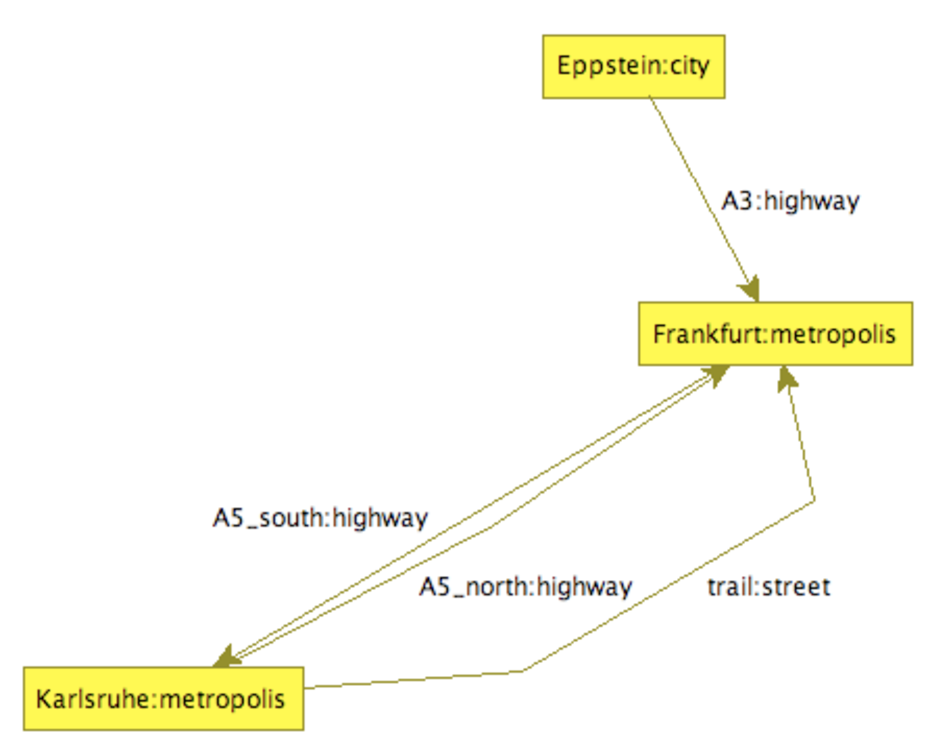
\includegraphics[width=8.5cm]{fig/map}}
\end{center}

This graph is valid, but not strict valid.
\lstset{language=grshell}
\begin{lstlisting} 
> validate
The graph is valid.
> validate strict
The graph is NOT valid:
  CAE: city "Eppstein" -- highway "A3" --> metropolis 
            "Frankfurt" not specified
  CAE: metropolis "Karlsruhe" -- street "trail" --> 
            metropolis "Frankfurt" not specified
>
\end{lstlisting}}

\begin{rail}
  'custom' 'graph' ( ( ) | SpacedParameters )
\end{rail}
Executes a command specific to the current backend. If \emph{SpacedParameters} is omitted, a list of available commands will be displayed (for the LGSP backend see \ref{custom}).

\subsection{Graph Manipulation Commands}
\label{mani}
In order to create graph elements an optional constructor can be used. 
\begin{rail}
  Constructor : '(' (() | (dollar '=' Text (() | ',' Attributes) | Attributes)) ')';
  Attributes : SingleAttribute + ',' ;
  SingleAttribute : AttributeName '=' TextOrNumber ; 
\end{rail}
A comma separated list of attribute declarations is supplied to the constructor. Available attribute names are specified by the graph model of the current working graph. All the undeclared attributes will be initialized with default values, depending on their type (int, enum $\leftarrow$ 0; boolean $\leftarrow$ false; String $\leftarrow$ ``'').\\
The \texttt{\$} marks a special attribute: an unique identifier of the new graph element. This identifier also is denoted as \emph{persistent name} (see \ref{persistentex}, \emph{GraphElement}). This name can be specified by a constructor only.

\begin{rail}
  'new' (() | Text) (() | ':' NodeType (() | Constructor))
\end{rail}
Creates a new node within the current graph. Optionally a variable \emph{Text} is assigned to the new node. If \emph{NodeType} is supplied, the new node will be of type \emph{NodeType} and attributes can be initialized by a constructor. Otherwise the node will be of the base node class type \emph{Node}.

\begin{rail}
  'new' Node '-' (()|Text) \\ (() | ':' EdgeType (() | Constructor)) '->' Node
\end{rail}
Creates a new edge within the current graph between the specified nodes, directed towards the second \emph{Node}. Optionally  a variable \emph{Text} is assigned to the new edge. If \emph{EdgeType} is supplied, the new edge will be of type \emph{EdgeType} and attributes can be initialized by a constructor. Otherwise the edge will be of the base edge class type \emph{Edge}.

\begin{rail}
  GraphElement '.' AttributeName '=' TextOrNumber
\end{rail}
Set the attribute \emph{AttributeName} of the graph element \emph{GraphElement} to the value of \emph{TextOrNumber}.

\begin{rail}
  'delete' 'node' Node
\end{rail}
Deletes the node \emph{Node} from the current graph. Incident edges will be deletes as well.

\begin{rail}
  'delete' 'edge' Edge
\end{rail}
Deletes the edge \emph{Edge} from the current graph.  
  
\subsection{Graph Query Commands}

\begin{rail}
  'show' 'num' ('nodes' (() | NodeType) | 'edges' (() | EdgeType))
\end{rail}
Gets the number of nodes/edges of the current graph. If a node type resp. edge type is supplied, only elements compatible to this type are considered.

\begin{rail}
  'show' ('nodes' (() | NodeType) | 'edges' (() | EdgeType))
\end{rail}
Gets the persistent names and the types of all the nodes / edges of the current graph. If a node type or edge type is supplied, only elements compatible to this type are considered. Nodes / edges without persistent names are shown with a pseudo-name.

\begin{rail}
  'show' ('node' | 'edge') 'types'
\end{rail}
Gets the node / edge types of the current graph model.

\begin{rail}
'show' ('node' ('super' | 'sub') 'types' NodeType | 'edge' ('super' | 'sub') 'types' EdgeType)
\end{rail}
Gets the inherited / descended types of \emph{NodeType} / \emph{EdgeType}.

\begin{rail}
  'show' ('node' 'attributes' (() | (() | 'only') NodeType) | 'edge' 'attributes' (() | (() | 'only') EdgeType))
\end{rail}
Gets the available node / edge attribute types. If \emph{NodeType} / \emph{EdgeType} is supplied, only attributes defined in \emph{NodeType} / \emph{EdgeType}. The \texttt{only} keyword excludes inherited attributes.\\
\textbf{Note:} This is in contrast to the \texttt{show num\dots}, \texttt{show nodes\dots} and \texttt{show edges\dots} commands where types and \emph{sub}types are specified.

\begin{rail}
 'show' ('node' Node | 'edge' Edge)
\end{rail}
Gets the attribute types and values of a specific graph element.

\begin{rail}
  'show' GraphElement '.' AttributeName
\end{rail}
Gets the value of a specific attribute.

\begin{rail}
  'node' 'type' Node 'is' Node | 'edge' 'type' Edge 'is' Edge
\end{rail}
Gets the information, whether the first element is type-compatible to the second element.

\subsection{Graph Output Commands}

\begin{rail}
  'save' 'graph' Filename
\end{rail}
Dumps the current graph as GrShell script into \emph{Filename}. The created script includes
\begin{itemize}
  \item selecting the backend
  \item creating all nodes and edges
  \item restoring the persistent names (see \ref{mani}),
\end{itemize}
but not necessarily using the same commands you typed in during construction.

\begin{rail}
  'show' 'graph' Filename (() | Text)
\end{rail}
Dumps the current graph as VCG formatted file into a temporary file. \emph{Filename} specifies an executable. The temporary VCG file will be passed to \emph{Filename} as last parameter. Additional parameters, such as program options, can be specified by \emph{Text}. If you use YComp as executable, this may look like
\begin{center}
  BILD (Dragon?)
\end{center}  
The temporary file will be deleted, when \emph{Filename} is terminated, if GrShell is still running at this time.

\begin{rail}
  'dump' 'graph' Filename
\end{rail}
Dumps the current graph as VCG formatted file into \emph{Filename}.\\
\\
The following commands control the style of the VCG output. This affects \texttt{dump graph}, \texttt{show graph} and \texttt{enable debug}. 
\begin{rail}
  'dump' 'set' ('color' | 'textcolor' | 'bordercolor') 'node' NodeType '=' Color
\end{rail}
Sets the color / text color / border color of the nodes of type \emph{NodeType}. This doesn't include sub types of \emph{NodeType}.

\begin{rail}
  'dump' 'set' ('color' | 'textcolor') 'edge' EdgeType '=' Color
\end{rail}
Sets the color / text color of the edges of type \emph{EdgeType}. This doesn't include sub types of \emph{NodeType}.

\begin{rail}
  'dump' 'add' 'exclude' 'node' NodeType
\end{rail}
Excludes nodes of type \emph{NodeType} (or sub type of \emph{NodeType}) as well as their incident edges from output.

\begin{rail}
  'dump' 'add' 'group' 'node' NodeType
\end{rail}
Declares \emph{NodeType} (or sub type of \emph{NodeType}) as group node type. All the different typed nodes that points to a node of type \emph{NodeType} (i.e.\ there is a directed edge between such nodes) will be grouped and visibly enclosed by the \emph{NodeType}-node.
The following example shows \emph{metropolis} ungrouped and grouped:
\begin{center}
  \fbox{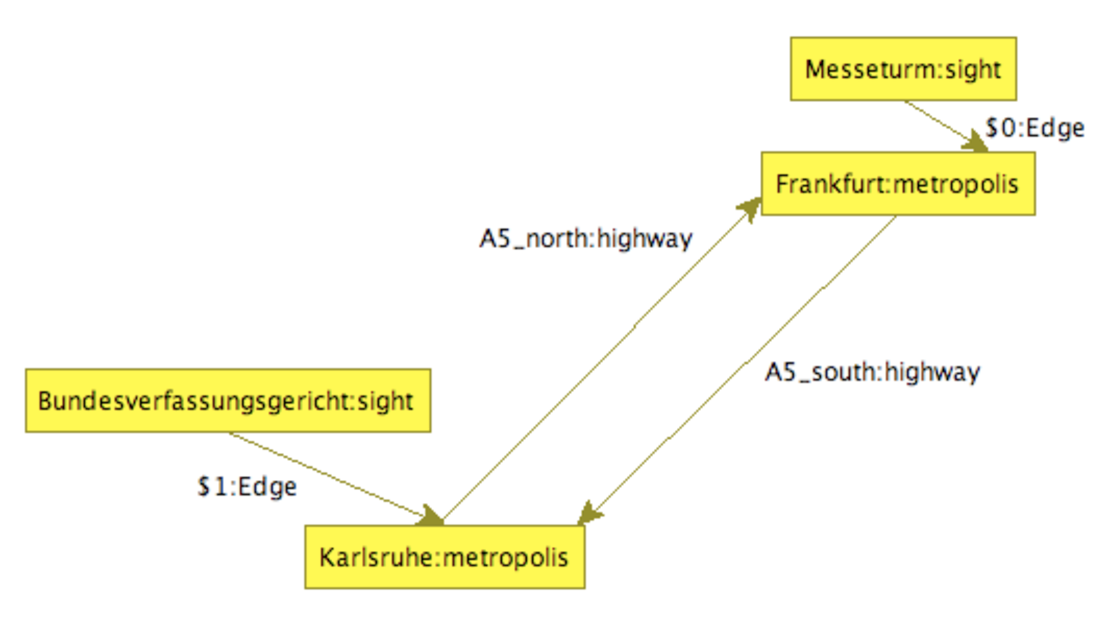
\includegraphics[width=0.45\linewidth]{fig/group1}}  \hfill \fbox{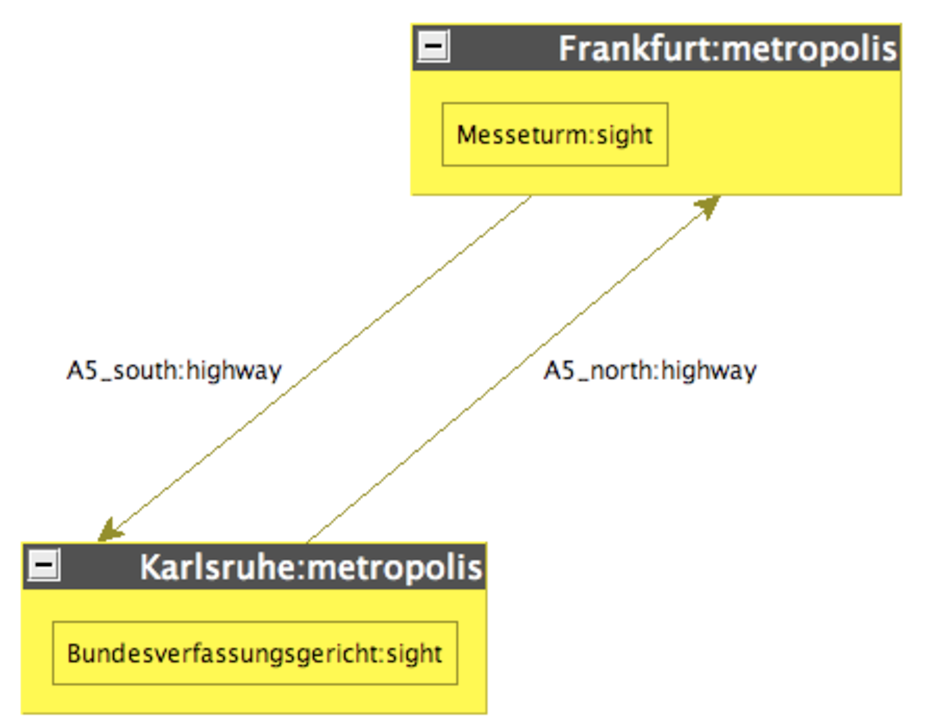
\includegraphics[width=0.45\linewidth]{fig/group2}}
\end{center}

\begin{rail}
  'dump' 'add' 'infotag' ('node' NodeType | 'edge' EdgeType) AttributeName
\end{rail}
Declares the attribute \emph{AttributeName} to be an ``info tag''. Info tags are displayed like additional node / edge labels. In the following example \emph{river} and \emph{jam} are info tags:
\begin{center}
  \fbox{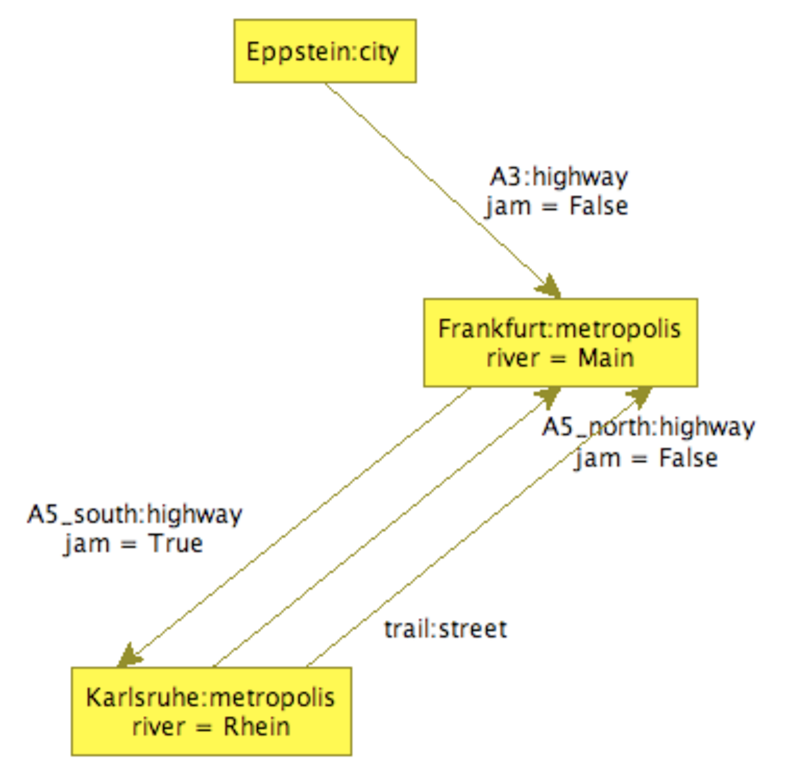
\includegraphics[width=0.7\linewidth]{fig/infotag}}
\end{center}


\begin{rail}
  'dump' 'set' 'edge' 'labels' ('on' | 'off')
\end{rail}
Specifies, whether edge labels will be displayed or not (default to ``on'').

\begin{rail}
  'dump' 'reset'
\end{rail}
Reset all style options (\texttt{dump set}\dots) to their default values.

\subsection{Action Commands}
An \emph{action} denotes a graph rewriting rule.

\begin{rail}
  'select' 'actions' Filename
\end{rail}
Selects a rule set. \emph{Filename} can be either a .NET assembly (e.g.\ ``rules.dll'') or a source file (``rules.cs''). Only one rule set can be loaded at once.

\begin{rail}
  'show' 'actions'
\end{rail}
Lists all the rules of the loaded rule set, their parameters and their return values. Rules can return a set of graph elements.

\begin{rail}
  'custom' 'actions' (() | SpacedParameters)
\end{rail}
Executes an action specific to the current backend. If \emph{SpacedParameters} is omitted, a list of available commands will be displayed (for the LGSPBackend see section \ref{custom}).

\subsubsection{Regular Graph Rewrite Sequences (GRS)}
Basically a graph rewriting command looks like this:
\makeatletter
\begin{rail}
  (() | 'debug') 'grs' SimpleRewriteSequence ;
  SimpleRewriteSequence: (SimpleTerm (() | ('*' | lbrace Number rbrace))) + ((() | dollar) (';' | '|' | ampersand));
  SimpleTerm: (() | '!') ('[' Rule ']' | Rule) |
    Text '=' (Text | '@' '(' Text ')') |
    'def' '(' Parameters ')' |
    'true' |
    'false' |
    '(' SimpleRewriteSequence ')' ;
  Rule: (() | '(' Parameters ')' '=') Action (() | '(' Parameters ')') ;
\end{rail}
\makeatother
\mbox{\quad}\\
Table \ref{ruletab} lists graph rewriting expressions at a glance. The operators hold the following order of precedence, starting with the lowest precedence: 
\[ \text{\texttt{;}} \;\;\;\;\;\;\; \text{\texttt{|}} \;\;\;\;\;\;\;  \text{\texttt{\&}}\] 
\makeatletter
\begin{table}[htbp]
\begin{tabularx}{\linewidth}{|lX|}
\hline
\texttt{s ; t}		& \textbf{Concatenation.} First, \texttt{s} is executed, afterwards \texttt{t} is executed. The sequence \texttt{s ; t} is \emph{successfully} executed iff \texttt{s} or \texttt{t} is successfully executed.\\
\texttt{s | t}		& \textbf{XOR.} First, \texttt{s} is executed. Only if \texttt{s} fails, \texttt{t} is executed. The sequence \texttt{s | t} is successfully executed iff \texttt{s} or \texttt{t} is successfully executed.\\
\texttt{s \& t}	& \textbf{Transactional AND.} First, \texttt{s} is executed, afterwards \texttt{t} is executed. If \texttt{s} or \texttt{t} fails, the action will be terminated and a rollback to the state before \texttt{s \& t} is performed.\\
\texttt{\$<op>}	& Flags the operator \texttt{<op>} as commutative. Usually operands are executed / evaluated from left to right with respect to bracketing (left-associative). But the sequences \texttt{s}, \texttt{t}, \texttt{u} in \texttt{s \$<op> t \$<op> u} are executed / evaluated in arbitrary order. \\
\texttt{s *}		& Executes \texttt{s} repeatedly as long as its execution does not fail.\\
\texttt{s \{n\}}	& Executes \texttt{s} repeatedly as long as its execution does not fail, but anyway \texttt{n} times at most.\\
\texttt{!}		& Found matches are dumped into VCG formatted files. [Die subgraphen?]\\
\texttt{\emph{Rule}} & Only the first pattern match produced by the action \emph{Rule} will be rewritten.\\
\texttt{[\emph{Rule}]} & Every pattern match produced by the action \emph{Rule} will be rewritten. \textbf{Note:} This operator is mainly added for benchmark purposes. Its semantic is not equal to \texttt{Rule*}. Instead this operator collects all the matches first before starting rewritings. In particular one needs to avoid deleting a graph element that is bound by another match. \\
\texttt{v = w}	& The variable \texttt{v} is assigned to \texttt{w}. If \texttt{w} is undefined, \texttt{v} will be undefined, too.\\
\texttt{v = @(x)}	& The variable \texttt{v} is assigned to the graph element identified by \texttt{x}. If \texttt{x} is not defined any more, \texttt{v} will be undefined, too.\\
\texttt{def(\emph{Parameters})} & Gets \emph{successful} if all the graph elements in \emph{Parameters} exist, i.e.\ if all the variables are defined.\\
\texttt{true}	& A constant acting as a successful match.\\
\texttt{false}	& A constant acting as a failed match.\\ \hline
\end{tabularx}\\
\\ \centering
{\small Let \texttt{s}, \texttt{t}, \texttt{u} be graph rewriting sequences, \texttt{v}, \texttt{w} variable identifiers, \texttt{x} an identifier of a graph element, \texttt{<op>} $\in \{\texttt{;}, \texttt{|}, \texttt{\&}\}$ and \texttt{n} $\in \N_0$.}
\caption{Graph rewriting expressions}
\label{ruletab}
\end{table}
\makeatother

Variables can be assigned to graph elements returned by rules using \texttt{(\emph{Para\-meters}) = \emph{Action}}. The desired variable identifiers have to be listed in \emph{Parameters}. Graph elements required by rules must be provided using \texttt{\emph{Action} (\emph{Para\-meters})}, where \emph{Parameters} is a list of variable identifiers. For undefined variables the specific element constraint of \emph{Action} will be ignored (every element matches).\\

Use the \texttt{debug} option to trace the rewriting process step-by-step. During execution YComp will display every single step. The debugger can be controlled by GrShell. The debug commands are shown in table \ref{tabdebug}.
\begin{table}[htbp]
  \begin{tabularx}{\linewidth}{|lX|} \hline
  \texttt{s}(tep) & Executes the next rewriting rule (match and rewrite)\\
  \texttt{d}(elaied step) & Executes a rewriting rule in a three-step procedure: matching, highlighting elements to be changed, doing rewriting \\
  \texttt{n}(ext) & Ascends one level up within the Kantorowitsch tree of the current rewrite sequence\\
  (step) \texttt{o}(ut) & Continues a rewriting sequence until the end of the current loop. If the execution is not in a loop at this moment, the complete sequence will be executed\\
  \texttt{r}(un) &  Continues execution without further stops\\
  \texttt{a}(bort) & Cancels the execution immediately\\ \hline 
  \end{tabularx}
  \caption{GrShell debug commands}
  \label{tabdebug}
\end{table}

\section{LGSPBackend Custom Commands}
\label{custom}
The LGSPBackend supports the following custom commands:

\subsection{Graph Related Commands}
\begin{rail}
  'custom' 'graph' analyzegraph
\end{rail}
Analyzes the current working graph. The analysis data provides vital information for efficient search plans. Analysis data are available as long as GrShell is running, i.e.\ when the working graph changes the analysis data is still available but maybe obsolete.

\subsection{Action Related Commands}
\begin{rail}
  'custom' 'actions' gensearchplan Action
\end{rail}
Creates a search plan for the rewriting rule \emph{Action} using a heuristic method and the analyze data (if the graph has been analyzed by \texttt{custom graph analyze\_graph}). Otherwise a default search plan is used. For efficiency reasons it is recommended to do analyzing and search plan creation during the rewriting procedure. Therefore the host graph should be in a stage similar to the final result. This is kind of a rough specification. In deed there might be some trial-and-error steps necessary to get a efficient search plan. A search plan is available as long as the current rule set remains loaded. 

\begin{rail}
  'custom' 'actions' setmaxmatches Number
\end{rail}
Sets the maximum amount of possible pattern matches to \emph{Number}. This command affects the expression \texttt{[\emph{Rule}]}. For \emph{Number} less or equal to zero, the constraint is reset.

\chapter{Examples}
\label{anexample}
\section{Busy Beaver}
We want \GrG\ to work as hard as a busy beaver \cite{kroll, bb}. Our busy beaver is a turing machine, that has got five states, writes 1,471 bars onto the tape and terminates \cite{beaver}. So first of all we design a turing machine as graph model. Besides this example shows that \GrG\ is turing complete. 

\subsection{Graph Model}
Let's start with
\lstset{language=grgenmodel}
\begin{lstlisting}[name=gr]
model TuringMashine;
\end{lstlisting}

The tape will be a chain of \emph{TapePosition} nodes connected by right edges. A cell value is modeled by a reflexive \emph{value} edge, attached to a \emph{TapePosition} node. The leftmost and the rightmost cell (\emph{TapePosition}) does not have an incoming and outgoing edge respectively. Therefore we have the node constraint $[0:1]$.
\lstset{language=grgenmodel}
\begin{lstlisting}[name=gr]
node class TapePosition; 
edge class right
  connect TapePosition[0:1] -> TapePosition[0:1];
  
edge class value
  connect TapePosition[1] -> TapePosition[1];  
edge class zero extends value;
edge class one extends value;
edge class empty extends value;  
\end{lstlisting}
Finally we need states and transitions. The current configuration is modeled with a \emph{RWHead} edge pointing to a \emph{TapePosition} node. \emph{State} nodes are connected with \emph{WriteValue} nodes via \emph{value} edges and from a \emph{WriteValue} node a \emph{move\dots} edge leads to the next state.
\begin{lstlisting}[name=gr]
node class RWHead;

node class WriteValue;
node class WriteZero extends WriteValue;
node class WriteOne extends WriteValue;
node class WriteEmpty extends WriteValue; 

edge class moveLeft;
edge class moveRight;
edge class dontMove;
\end{lstlisting}

\subsection{Rule Set}
Now the rule set: we start with
\lstset{language=grgenactions}
\begin{lstlisting}[name=grg] 
actions Turing using TuringModel;
\end{lstlisting}
We need rewrite rules for the following steps of the turing machine:
\begin{enumerate}
  \item Reading the value of the current tape cell and select a outgoing edge of the current state.
  \item Writing a new value in the current cell, according to the sub type of the \emph{WriteValue} node.
  \item Move the read-write-head along the tape and propagate a new state as current state. 
\end{enumerate}
As you can see a transition of the turing machine is split into two graph rewriting steps: Writing the new value onto the tape and performing the state transition. We need eleven rules, three rules for each step (for ``zero'', ``one'' and ``empty'') and two rules for extending the tape to the left and the the right, respectively.
\begin{lstlisting}[name=grg] 
rule readZeroRule {
	pattern {
		s:State -:RWHead->tp:TapePosition -zv:zero->tp;
		s -zr:zero-> wv:WriteValue;
	}
	replace {
		s -zr-> wv;
		tp -zv-> tp;
		wv -:RWHead->tp;
	}
}      
\end{lstlisting}
We the state and the current cell (\emph{RWHead} edge) and check, if the cell value is zero. Furthermore we check, if the state has a transition for zero. The replacement part deletes the \emph{RWHead} edge between \emph{s} and \emph{tp} and adds it between \emph{wv} and \emph{tp}. Analogous the remaining rules:
\begin{lstlisting}[name=grg] 
rule readOneRule {
	pattern {
		s:State -:RWHead-> tp:TapePosition -ov:one-> tp;
		s -or:one-> wv:WriteValue;
	}
	replace {
		s -or-> wv;
		tp -ov-> tp;
		wv -:RWHead-> tp;
	}
}

rule readEmptyRule {
	pattern {
		s:State -:RWHead-> tp:TapePosition -ev:empty-> tp;
		s -er:empty-> wv:WriteValue;
	}
	replace {
		s -er-> wv;
		tp -ev-> tp;
		wv -:RWHead-> tp;
	}
}

rule writeZeroRule {
	pattern {
		wv:WriteZero -rw:RWHead-> tp:TapePosition -:value-> tp;
	}
	replace {
		wv -rw-> tp -:zero-> tp;
	}	
}

rule writeOneRule {
	pattern {
		wv:WriteOne -rw:RWHead-> tp:TapePosition -:value-> tp;
	}
	replace {
		wv -rw-> tp -:one-> tp;
	}	
}

rule writeEmptyRule {
	pattern {
		wv:WriteEmpty -rw:RWHead-> tp:TapePosition -:value-> tp;
	}
	replace {
		wv -rw-> tp -:empty-> tp;
	}	
}

rule moveLeftRule {
	pattern {
		wv:WriteValue -m:moveLeft-> s:State;
		wv -:RWHead-> tp:TapePosition <-r:right- ltp:TapePosition;
	}
	replace {
		wv -m-> s;
		s -:RWHead-> ltp -r-> tp;
	}
}

rule moveRightRule {
	pattern {
		wv:WriteValue -m:moveRight-> s:State;
		wv -:RWHead-> tp:TapePosition -r:right-> rtp:TapePosition;
	}
	replace {
		wv -m-> s;
		s -:RWHead-> rtp <-r- tp;
	}
}

rule dontMoveRule {
	pattern {
		wv:WriteValue -m:dontMove-> s:State;
		wv -:RWHead-> tp:TapePosition;
	}
	replace {
		tp;
		wv -m-> s;
		s -:RWHead-> tp;
	}
}

rule ensureMoveLeftValidRule {
	pattern {
		wv:WriteValue -m:moveLeft-> s:State;
		wv -rw:RWHead-> tp:TapePosition;
		negative {
			tp <-:right- ltp:TapePosition;
		}
	}
	replace {
		wv -m-> s;
		wv -rw-> tp <-:right- ltp:TapePosition -:empty-> ltp;
	}
}

rule ensureMoveRightValidRule {
	pattern {
		wv:WriteValue -m:moveRight-> s:State;
		wv -rw:RWHead-> tp:TapePosition;
		negative {
			tp -:right-> rtp:TapePosition;
		}
	}
	replace {
		wv -m-> s;
		wv -rw-> tp -:right-> rtp:TapePosition -:empty-> rtp;
	}
}
\end{lstlisting}
Have a look at the negative condition within the \emph{ensureMove\dots} rules. They ensure, that the current cell is in deed at the end of the tape: an edge to a right / left neighbor cell may not exist.

Finally we construct the busy beaver and let it work with GrShell:
\lstset{language=grshell}
\begin{lstlisting}[name=bb] 
select backend "lgspBackend.dll"
new graph "../lib/lgsp-TuringModel.dll" "Busy Beaver"
select actions "../lib/lgsp-TuringActions.dll"

# Initialize tape
new tp:TapePosition($="Startposition")

# States
new sA:State($="A")
new sB:State($="B")
new sC:State($="C")
new sD:State($="D")
new sE:State($="E")
new sH:State($ = "Halt")

new sA -:RWHead-> tp

# Transitions: three lines per state for
#   - updating cell value
#   - moving read-write-head
# respectively

new sA_0: WriteOne
new sA -:empty-> sA_0
new sA_0 -:moveLeft-> sB

new sA_1: WriteOne
new sA -:one ->sA_1
new sA_1 -:moveLeft->sD

new sB_0: WriteOne
new sB -:empty-> sB_0
new sB_0 -:moveRight-> sC

new sB_1: WriteEmpty
new sB -:one-> sB_1
new sB_1 -:moveRight-> sE

new sC_0: WriteEmpty
new sC -:empty ->sC_0
new sC_0 -:moveLeft->sA

new sC_1: WriteEmpty
new sC -:one-> sC_1
new sC_1 -:moveRight-> sB

new sD_0: WriteOne
new sD -:empty ->sD_0
new sD_0 -:moveLeft->sE

new sD_1: WriteOne
new sD -:one-> sD_1
new sD_1 -:moveLeft-> sH

new sE_0: WriteOne
new sE -:empty ->sE_0
new sE_0 -:moveLeft->sC

new sE_1: WriteOne
new sE -:one-> sE_1
new sE_1 -:moveLeft-> sC
}      
\end{lstlisting}

Our busy beaver looks like this:
\begin{center}
  \fbox{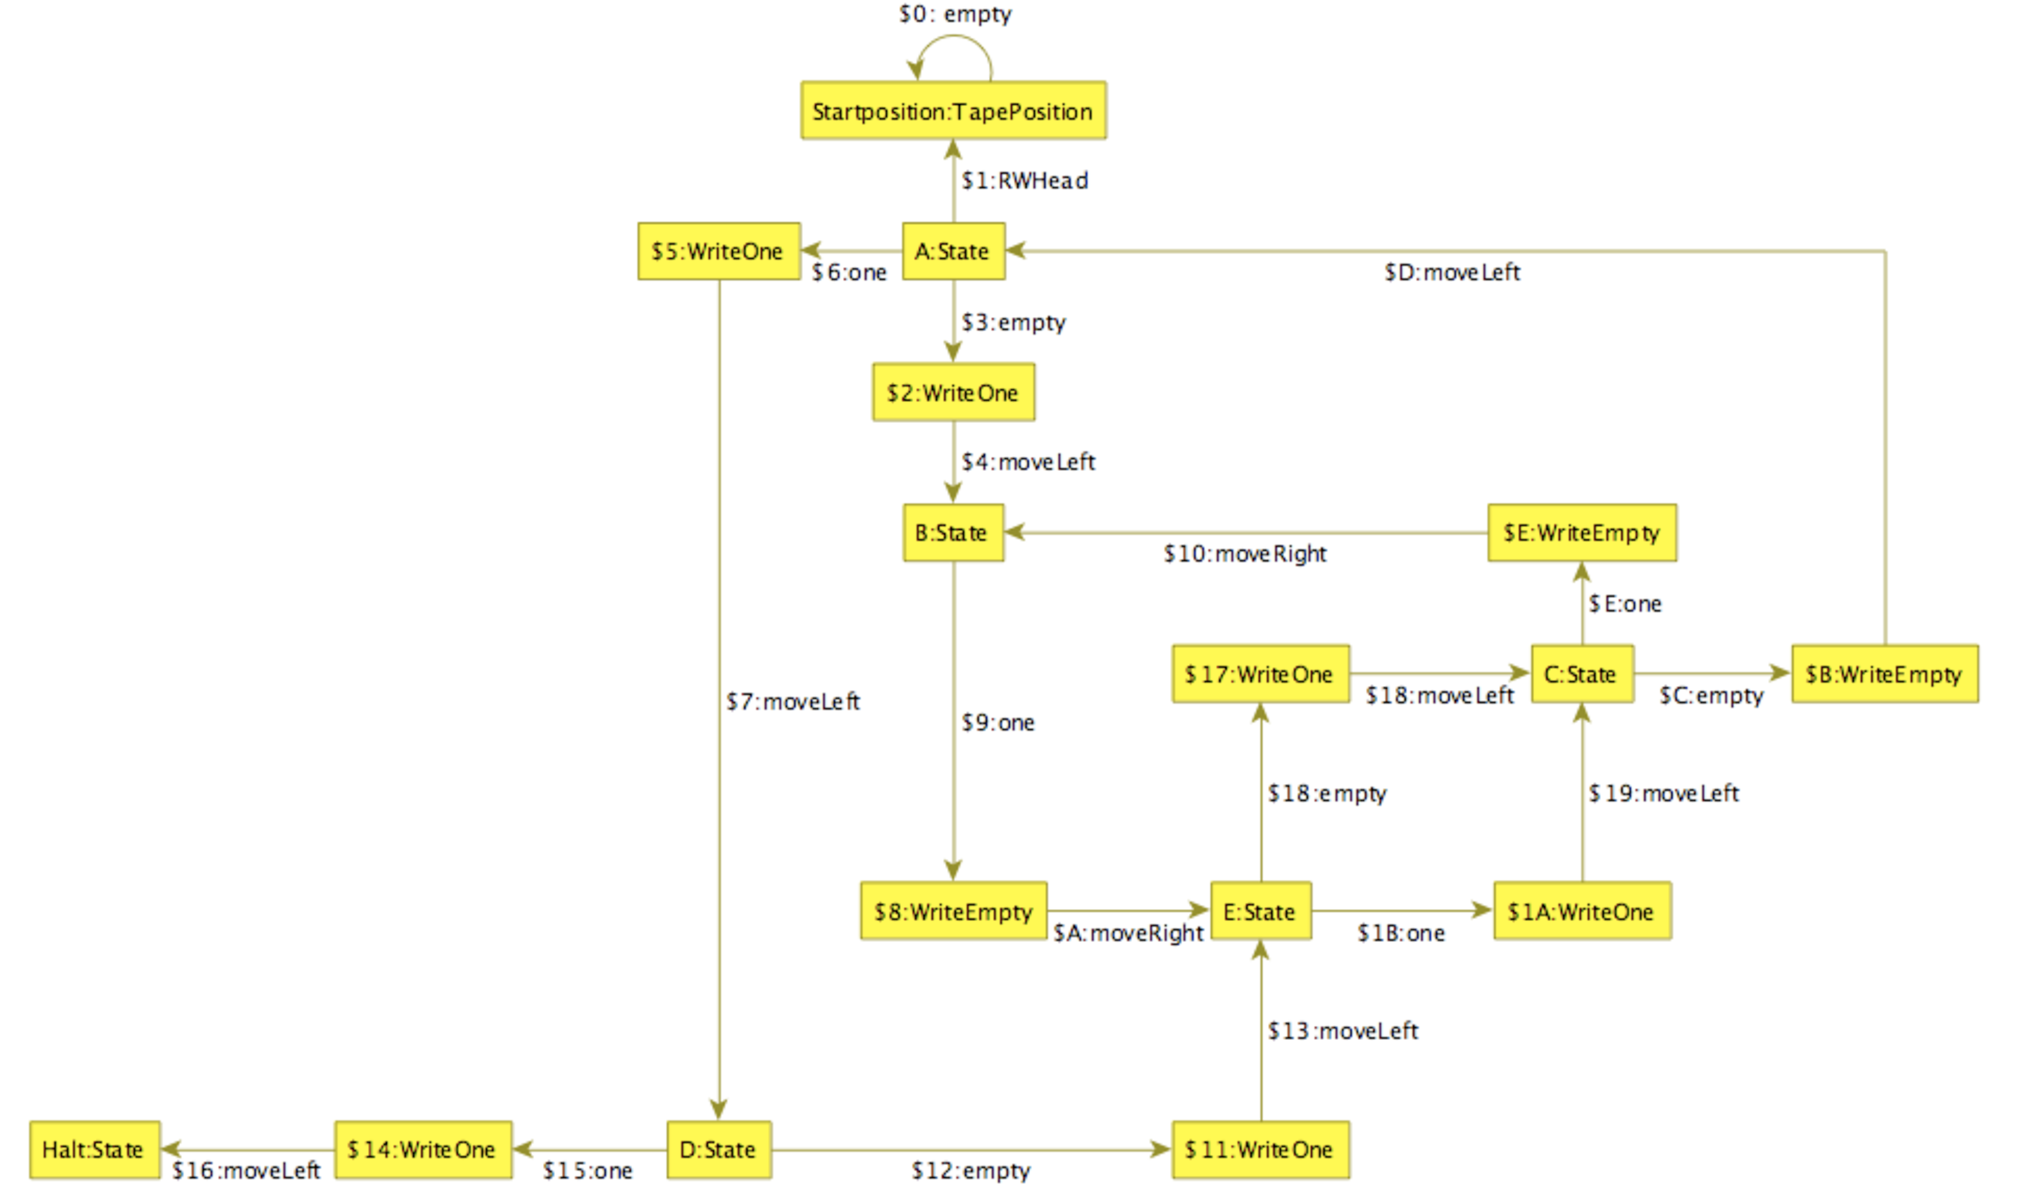
\includegraphics[width=\linewidth]{fig/bbstart}}
\end{center}
The graph rewriting sequence is quite straight forward and generic to the turing graph model. Note that for each state the ``\emph{\dots Empty\dots} | \emph{\dots One\dots}'' selection is unambiguous.
\begin{lstlisting}[name=bb]
  grs ((readOneRule | readEmptyRule) ; (writeOneRule | writeEmptyRule) ; (ensureMoveLeftValidRule | ensureMoveRightValidRule) ; (moveLeftRule | moveRightRule)){32}
\end{lstlisting}
We intercept the machine after 32 iterations and look at the result so far:
\begin{center}
  \fbox{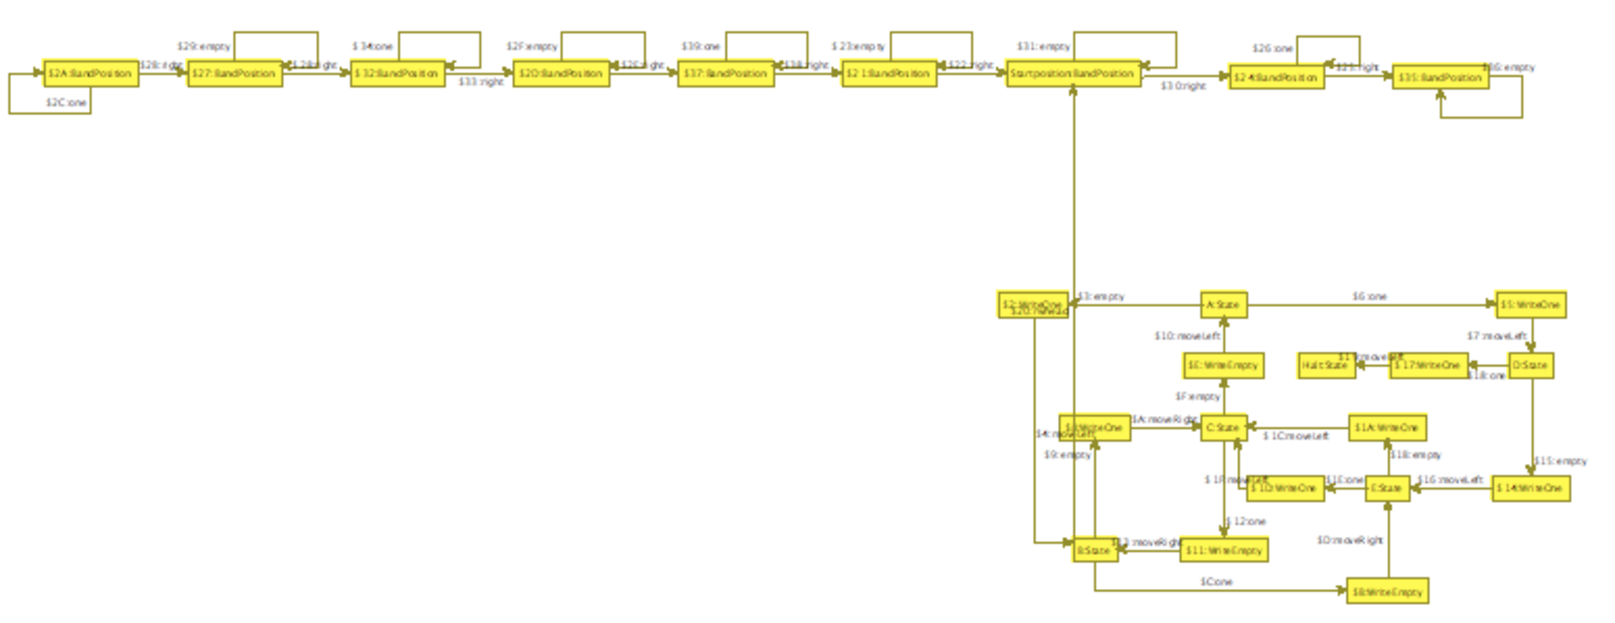
\includegraphics[width=\linewidth]{fig/bbmiddle}}
\end{center}
In order to improve the performance we generate better search plans.
\begin{lstlisting}[name=bb]
custom graph analyze_graph
custom actions gen_searchplan readOneRule
custom actions gen_searchplan readEmptyRule
custom actions gen_searchplan writeOneRule
custom actions gen_searchplan writeEmptyRule
custom actions gen_searchplan ensureMoveLeftValidRule
custom actions gen_searchplan ensureMoveRightValidRule
custom actions gen_searchplan moveLeftRule
custom actions gen_searchplan moveRightRule
\end{lstlisting}

Let the beaver run:
\begin{lstlisting}[name=bb]
  grs ((readOneRule | readEmptyRule) ; (writeOneRule | writeEmptyRule) ; (ensureMoveLeftValidRule | ensureMoveRightValidRule) ; (moveLeftRule | moveRightRule))*
\end{lstlisting}

\section{Fractals}

\thebibliography{99}
\bibitem{geiss} R. Geiß et al.: \emph{\GrG: A Fast SPO-Based Graph Rewriting Tool} in Graph Transformations, number 4178 in LNCS, pages 383-397, Springer, 2006
\bibitem{kroll} M. Kroll: \emph{Portierung des C-Anteils des Graphersetzungssystems \GrG\ nach C\# mit Erweiterungen}, Studienarbeit, Fakultät für Informatik, Universität Karlsruhe, 2007
\bibitem{hack} S. Hack: \emph{Graphersetzung für Optimierung in der Codeerzeugung} Diplomarbeit, Fakultät für Informatik, Universität Karlsruhe, 2003
\bibitem{grund} D. Grund: \emph{Negative Anwendungsbedingungen für den Graphersetzer \GrG} Studienarbeit, Fakultät für Informatik, Universität Karlsruhe, 2004 
\bibitem{adam} A. Szalkowski: \emph{Negative Anwendungsbedingungen für das suchprogrammbasierte Backend von GrGen} Studienarbeit, Fakultät für Informatik, Universität Karlsruhe, 2005
\bibitem{batz} G. Batz: \emph{Graphersetzung für eine Zwischendarstellung im Übersetzerbau} Diplomarbeit, Fakultät für Informatik, Universität Karlsruhe, 2005
\bibitem{pascal} K. Jensen, N. Wirth: \emph{Pascal User Manual and Report} Springer, $^41991$
\bibitem{bb} A. Dewdney: \emph{A computer trap for the Busy Beaver, the hardest-working machine} Scientific American, 251(2), pages 10-12, 16, 17, August 1984
\bibitem{beaver} H. Marxen, J. Buntrock: \emph{Old list of record TMs.}\\ http://www.drb.insel.de/~heiner/BB/index.html. Version: August 2000

\end{document}

\begin{figure}[htbp]
  \centering
  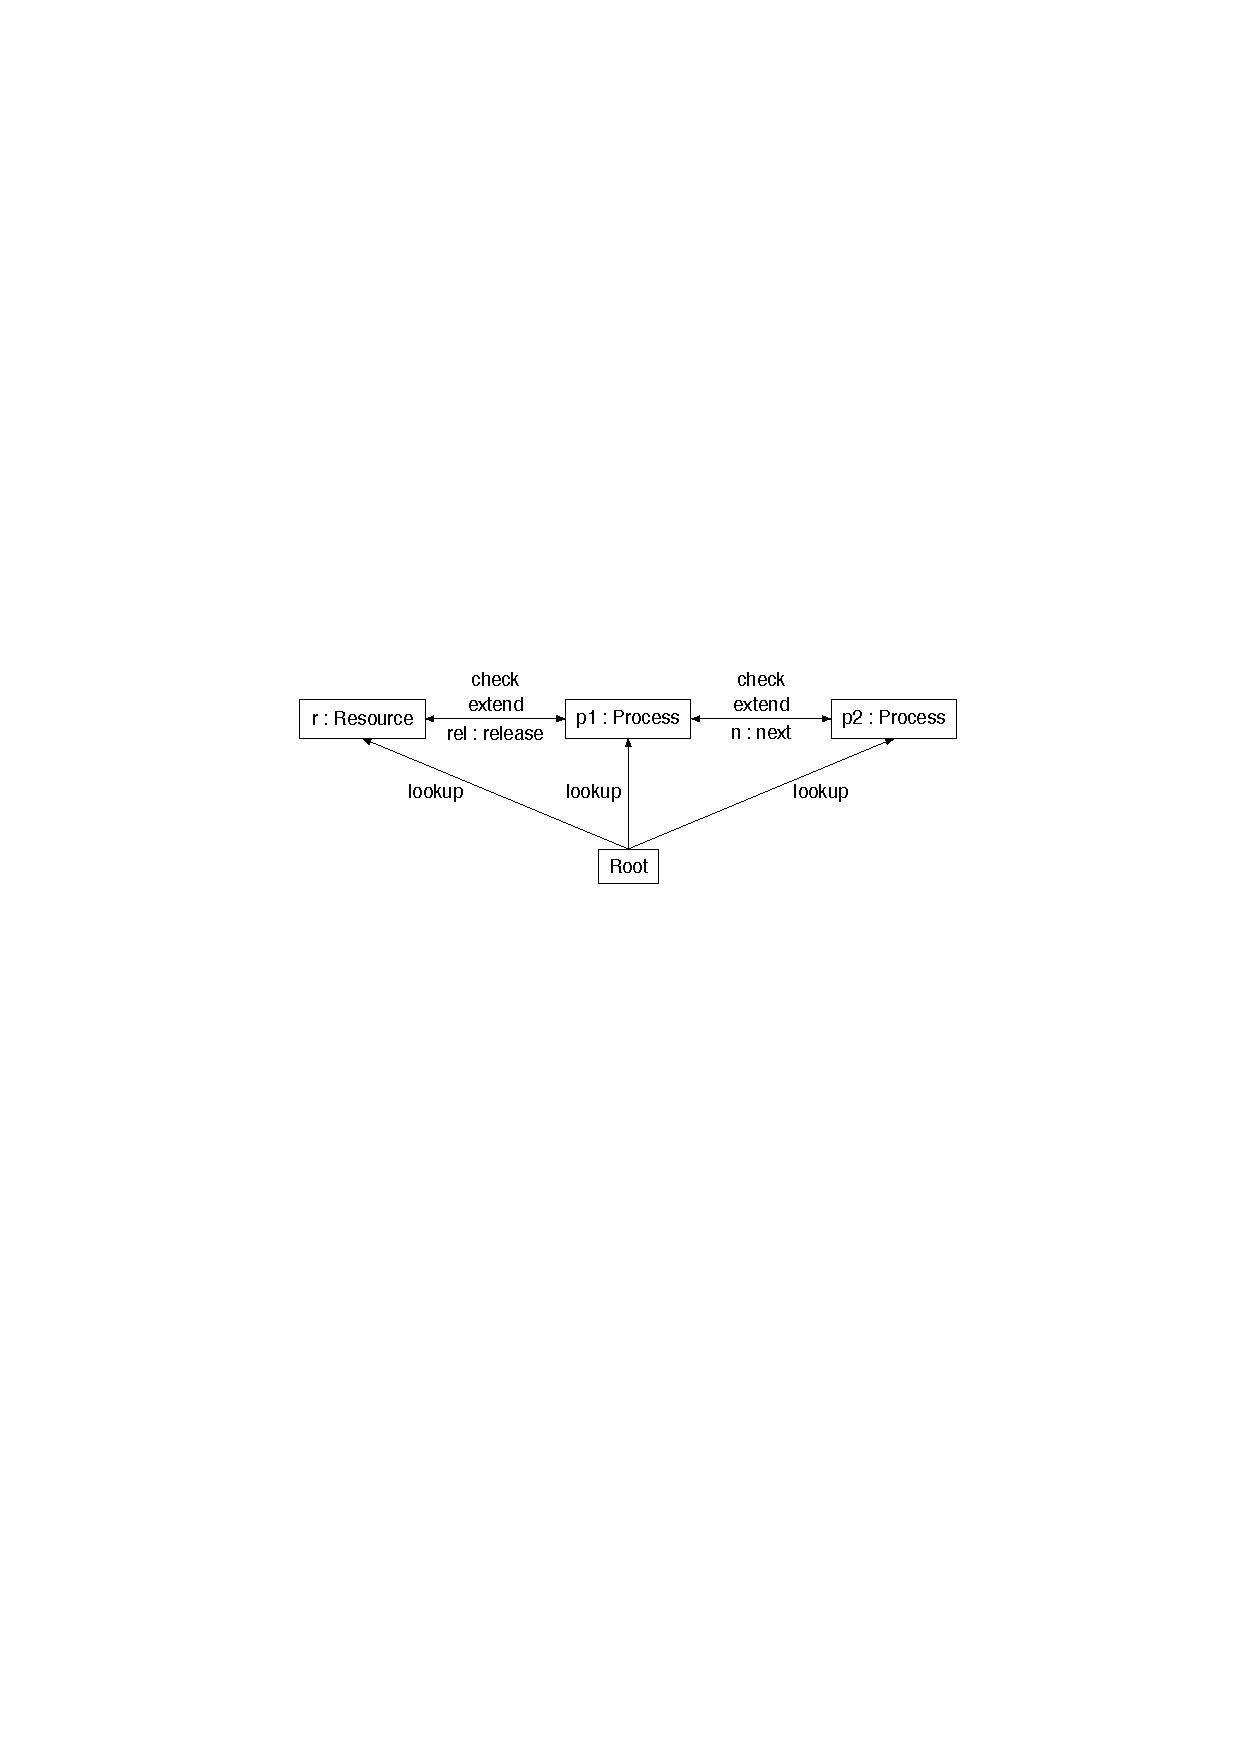
\includegraphics[width=0.7\linewidth]{fig/host}\\
  \footnotesize{Host graph $H$}\\
  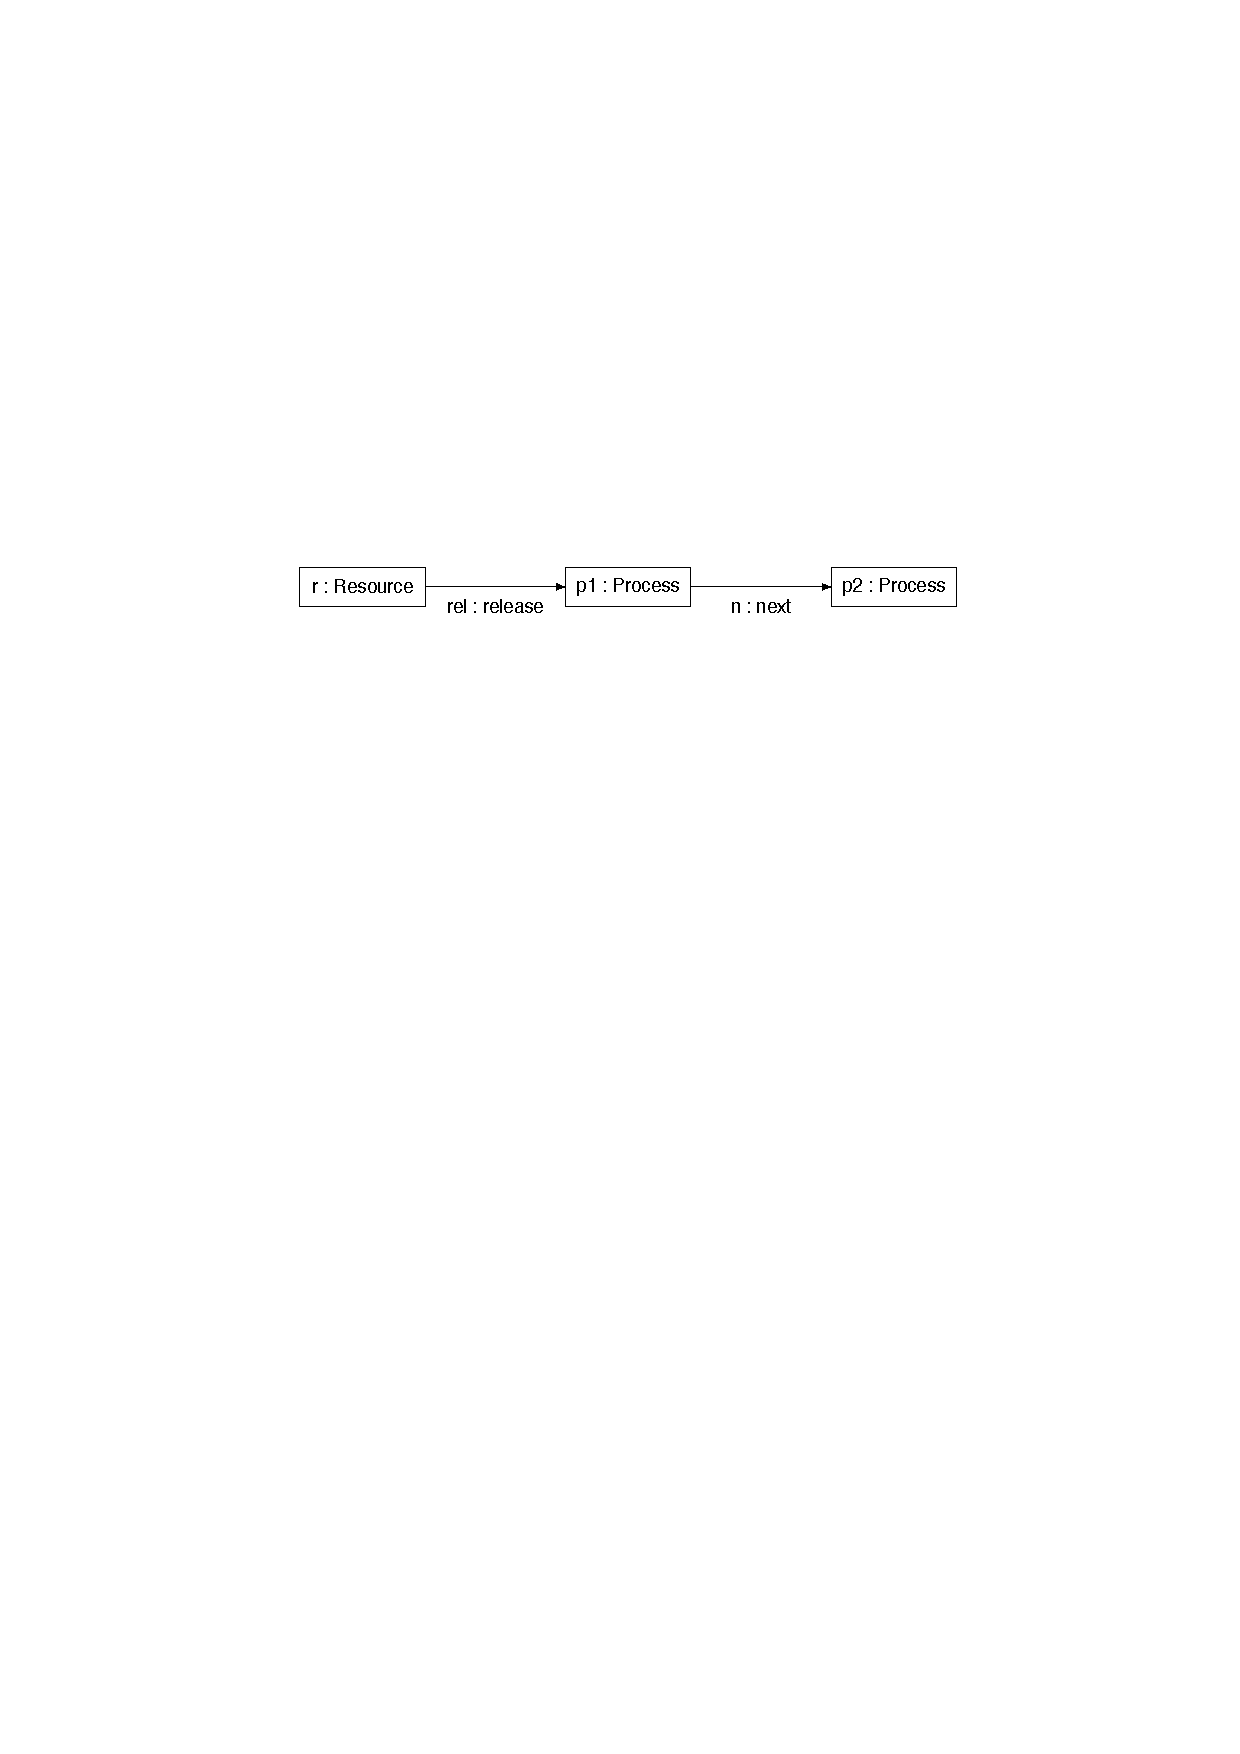
\includegraphics[width=0.7\linewidth]{fig/pattern}\\
  \footnotesize{Pattern graph $L$}\\
  \caption{A host graph and pattern graph. \cite{kroll}}
  \label{firstexample}
\end{figure}
